\section{Technologien}
\subsection{Databus[EK]}
\subsubsection{Allgemein}
Databus ist ein von LinkedIn entwickeltes Tool, welches sich selbst mit den Attributen „source-agnostic distributed change data capture system“ beschreibt. Als Open-Source Software wurde diese im Jahre 2013 unter der Apache-2.0 Lizenz der GitHub-Community bereitgestellt. 
(vgl. \cite{Databus-GitHub})
\vspace{5mm}\par
\textit{Source-Agnostic} bedeutet, dass Databus im Gegensatz zu einer Spezialisierung auf eine bestimmte Datenquelle, wie zum Beispiel ein bestimmter Typus von Datenbanken, darauf ausgelegt ist, ein breitgefächertes Spektrum an Datenquellen abzudecken. Damit soll die Unabhängigkeit von den Datenquellen gewährleistet werden.
\vspace{5mm}\par
\textit{Distributed} heißt, dass es sich bei Databus um ein verteiltes System handelt, welches sich die Vorteile von mehreren Computersystem zu Nutze machen kann und somit nicht auf ein singuläres System angewiesen ist.
\vspace{5mm}\par
\textit{Change-Data-Capture} (CDC) beschreibt einen Prozess, bei welchem die Änderung in einer Datenquelle - oft einer Datenbank - identifiziert und festgehalten wird. Diese gewonnen Änderungen werden dann an andere Systemarchitekturen, wie zum Beispiel ETL-Prozessen, zur Weiterverarbeitung zur Verfügung gestellt.
(vgl. \cite{CDC})
\newpage
\subsubsection{Wie funktioniert Databus?}
\begin{figure}[H]
    \centering
    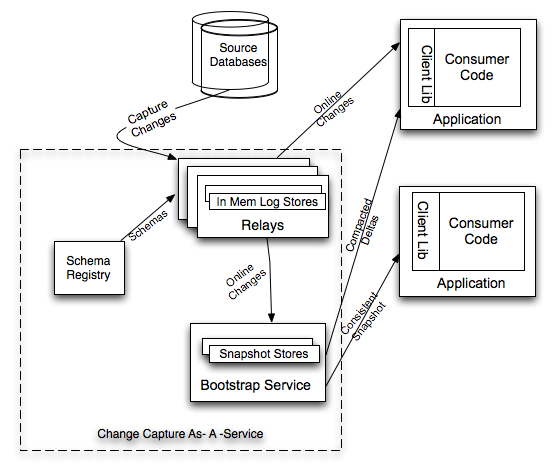
\includegraphics[scale=0.4]{images/databus-as-a-service.png}
    \caption{Databus-Aufbau (02.04.2020)}
    \label{img:}
    \url{http://s3.amazonaws.com/snaprojects/databus/databus-as-a-service.png}
\end{figure}
Wie man in der oben aufgezeigten Grafik sehen kann, besteht Databus aus folgenden drei Teilen: 
\begin{enumerate}
  \item \textbf{Relais:} Nimmt die aufgezeichneten Änderungen in der Datenquelle entgegen. Diese Änderungen werden in einem in-memory Log-Store abgespeichert, da dieser über die nötigen high-performance Eigenschaften verfügt.
  \item \textbf{Bootstrap-Service:} Periodisch nimmt dieser Daten des Relais entgegen. Ermöglicht wird dies durch eine periodische Umlenkung des Relais-Datenstroms auf den Bootstrap-Service. Dieser Service speichert die erhaltenen Daten dann als sogenannten Snapshot - eine Momentaufnahme der Daten zu einem bestimmten Zeitpunkt - ab.
  \item \textbf{Client-Library:} Diese wird in die Applikation eingefügt, um Daten aus dem Relais oder Bootstrap-Service erhalten zu können.
\end{enumerate}
Sollte der Fall eintreten, dass ein Consumer - eine Applikation, welche die Client-Library verwendet - datentechnisch zeitlich zurückfällt, so dass die benötigten Daten im Relais nicht länger vorliegen, kommt es zu folgendem Fall: ein konsolidierter Snapshot wird dem zurückliegenden Consumer übergeben, welcher diesen wieder auf Kurs bringt. Ähnlich sieht der Fall aus, wenn sich einer neuer Consumer einklinkt. Der Bootstrap-Service stellt auch in diesem Fall einen Snapshot bereit, welcher es dem Consumer ermöglicht, auf den aktuellen Stand zu kommen.
(vgl. \cite{Databus-Open-Sourcing})
\subsubsection{Entscheidungsprozess}
In der ersten Phase der Arbeit, sozusagen der Aneignungsphase, war Databus noch im Technologie-Stack enthalten. Anfangs wirkte das Tool vielversprechend für die Firma, durch Aspekte wie die freie Verfügbarkeit als Open-Source Software und damit die Möglichkeit eines Einblicks in dessen Funktionsweise. Doch bei weiterer Einarbeitung und Kenntnisnahme über die genaue Funktionalität, wurde die Verwendung von Databus auf Eis gelegt. Für die Firma MIC ist die Tatsache, dass man für die Verwendung von Databus jede Tabelle, welche auf Änderung beobachtet wird, abändern muss, ein Problem. Der Grund dafür liegt an der Menge der Tabellen, welche abgeändert werden müssten und dass ein solches Vorgehen nicht dem Echtzeitbetrieb vereinbar ist.

\subsubsection{Die Problematik verwahrloster Open-Source Software}
Wenn eine zuvor intern in Unternehmen entwickelte Software den Schritt macht, in den Open-Source Bereich entlassen zu werden, dann oft mit der Hoffnung, durch größere Beteiligung der Community und auch anderer Unternehmungen am Ende eine bessere Software zu erhalten, als wenn diese inhouse entwickelt worden wäre.
\vspace{5mm}\par
Dies beschreibt allerdings nur den Optimalfall. Durch die schnellen Veränderungen in einer Branche wie dieser kann es schnell zu Problemen bei der Nutzbarkeit der Software kommen, wenn diese nicht regelmäßig gewartet wird.So auch der Fall bei Databus, selbst die Replikation der auf GitHub präsentierten Beispiele war nur durch externe fremdsprachige Ressourcen möglich. Somit ist ein deutlich größerer Zeitaufwand  nötig, welcher nur schwer im voraus zu kalkulieren ist. Ohne also eine große Code-Kenntnis der Software kann ein solches Unterfangen schnell zu einer Gefahr werden, wenn längerfristig Projekte darauf aufgebaut werden sollen. 
\newpage
\subsection{Kafka[EK]}
\begin{figure}[H]
    \centering
    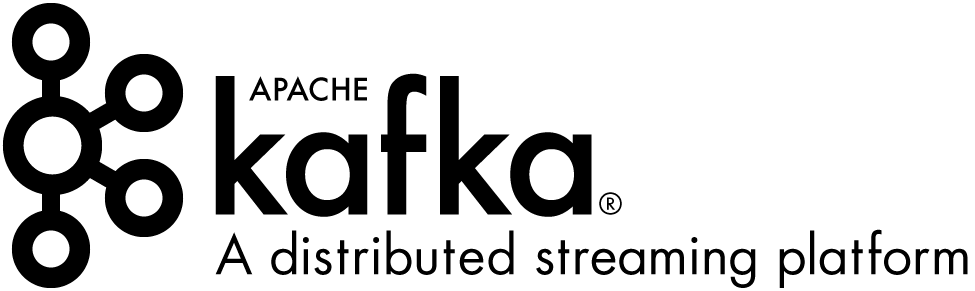
\includegraphics[scale=0.4]{images/kafka_logo.png}
    \caption{Kafka Logo (02.04.2020)}
    \url{https://kafka.apache.org/images/logo.png}
\end{figure}
\subsubsection{Allgemein}
Bei Kafka handelt es sich um eine verteilte Streaming-Plattform, welche von LinkedIn im Jahre 2011 als Open-Source Projekt veröffentlicht wurde. 
(vgl. \cite{Kafka-Open-Sourcing})Durch den Apache Incubator kam das Projekt im Jahre 2012 in die Hände der Apache Software Foundation und wird seitdem auch von Apache weiterentwickelt und gewartet.
(vgl. \cite{Kafka-Apache-Incubator})
\vspace{5mm}\par
Als Streaming-Plattform deckt Kafka drei Funktionalitäten ab.
Erste wäre das Ver-öffentlichen und Abonnieren von Record-Streams (Kafkas Bezeichnung für einen Datenstrom), ähnlich zu einem Enterprise-Messaging-System (EMS). Zweite wäre das Speichern von solchen Record-Streams, in einer Weise, in welcher diese dauerhaft fehlertolerant erfolgen. Dritte wäre die Verarbeitung von Streams im Moment des Auftretens.
\vspace{5mm}
Kafka soll vor allem diesen zwei Klassen von Applikationen zur Seite stehen:
\begin{itemize}
    \item Echtzeit Streaming-Data-Pipelines, welche zuverlässig Daten zwischen System oder auch Applikationen transportieren.
    \item Echtzeit Streaming-Applikationen, welche auf Daten-Streams reagieren oder diese transformieren.
\end{itemize}
(vgl. \cite{Kafka-Introduction})

\subsubsection{Wie funktioniert Kafka?}
Kafka wird als ein sogenannter Cluster auf einem oder mehreren Servern ausgeführt. 
\vspace{5mm}\par
Ein Cluster ist: „Eine Gruppe von unabhängigen Servern (üblicherweise in unmittelbarer Nähe zu einander), welche durch ein dediziertes Netzwerk vernetzt als eine zentralisierte Datenverarbeitungsressource arbeiten“
\cite{Cluster-Definition}
\newpage
Dieser Cluster speichert dann die Record-Streams in sogenannten Topics - die Kategorien für die Aufzeichnungen. Jede dieser Aufzeichnungen beziehungsweise Records steht aus dreierlei Bestandteilen: dem Key (eindeutige Identifikation), dem dazugehörigen Value (Wert) und einem Zeitstempel. Für das Management dieser Cluster verwendet Kafka Zookeeper.
\begin{figure}[H]
    \centering
    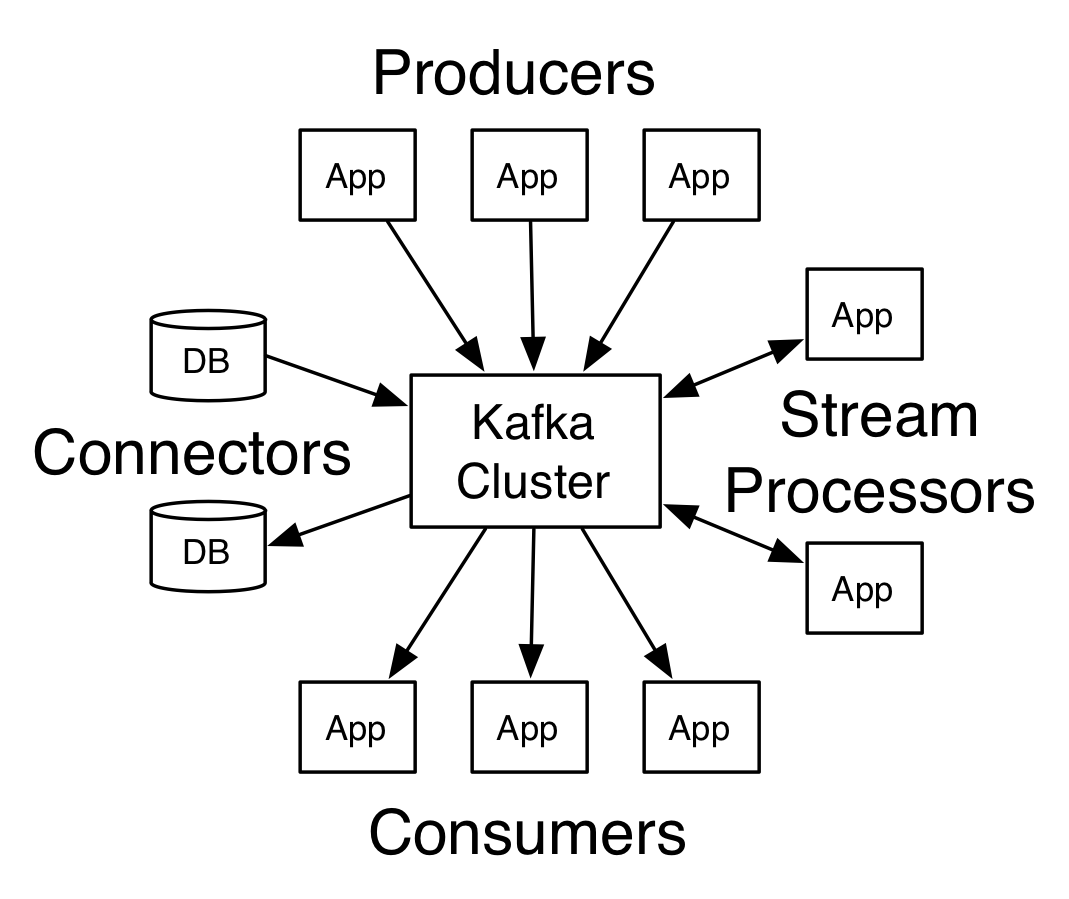
\includegraphics[scale=1.5]{images/kafka-apis.png}
    \caption{Kafka APIs (02.04.2020)}
    \url{https://kafka.apache.org/23/images/kafka-apis.png}
\end{figure}
Wie in der vorhergehenden Grafik zu sehen ist, bilden vier Core-APIs Kafka:
\begin{enumerate}
  \item \textbf{Producer API:} Will eine Applikation einen Record-Stream an den Kafka-Cluster und damit an ein Topic senden, so kann sie dies über diese API lösen.
  \item \textbf{Consumer API:} Bildet das Gegenstück zur Producer API; will eine Applikation zu einem bestimmten Topic zugehörige gesendete Record-Streams haben, muss jene einfach dieses Topic abonnieren.
  \item \textbf{Stream API: } Nimmt die beiden vorangegangen API-Funktionen Eins und Zwei an. Somit kann eine Applikation als ein Stream-Prozessor agieren, welcher sowohl den Input-Stream eines Topics konsumiert, als auch den Output-Stream zu einem anderen Topic liefert. So kann diese API einen Input-Stream zu einem Output-Stream transformieren.
  \item \textbf{Connector API:} Soll die Möglichkeit, geben bereits vorhanden Systeme und Applikationen mit einem Kafka-Topic zu verbinden, dies kann einerseits als Consumer und andererseits auch als Producer erfolgen. Ein Beispiel für einen Producer  wäre, wenn jede Änderung einer Datenbanktabelle aufgezeichnet werden soll und über den Kafka-Cluster für eine Weiterverarbeitung bereitstehen soll.
\end{enumerate}
Die APIs erlauben darüber hinaus, nicht nur die Verarbeitung eines Topics. Alle beschriebenen Funktionalitäten sind auch mit mehreren Topics möglich.
(vgl. \cite{Kafka-Introduction})
\subsubsection{Entscheidungsprozess}
Die Echtzeit-Komponente von Kafka ist ein tragender Grund für die Verwendung in dieser Arbeit, dies ermöglicht den Komponenten ohne größeren Zeitverlust die weiterzugebenden Daten mit der nachfolgenden Komponente zu kommunizieren. Des weiteren handelte es sich bei Kafka um eine Vorgabe der Firma MIC.

\subsection{ZooKeeper[EK]}
\begin{figure}[H]
    \centering
    
\includegraphics[scale=0.25]{images/zookeeper-logo.png}
    \caption{ZooKeeper Logo (02.04.2020)}
    \url{https://upload.wikimedia.org/wikipedia/en/thumb/8/81/Apache_ZooKeeper_Logo.svg/403px-Apache_ZooKeeper_Logo.svg.png}
\end{figure}
\subsubsection{Allgemein}
ZooKeeper ist eine Open-Source Software, welche von Freiwilligen unter dem Dach der Apache Software Foundation entwickelt wird. Ziel des Projektes ist es, einen Server, der eine sehr zuverlässige Koordination von verteilten System ermöglicht, bereitzustellen. 
(vgl. \cite{Apache-ZooKeeper})
\subsubsection{Nutzen für Kafka}
Beim Management der Cluster für Kafka fallen die folgenden Aufgaben an ZooKeeper. Die Koordinierung von Brokern. Das Bereitstellen von einem konsistenten Dateisystems für die Konfigurationsdateien. Die Auswahl eines sogenannten „Broker Topic Partition Leaders”.
(vgl. \cite{Kafka-Architecture})

\subsubsection{Funktionsweise}
Die interne Datenstruktur von ZooKeeper ähnelt einem Baum, heißt von dem Ausgangspunkt beziehungsweise der Wurzel erreichen wir alle weiteren Elemente über eine direkte Verbindung oder über deren übergeordneten Elemente. Jedes Element in diesem Baum ist ein Knoten, eine sogenannte zNode (z steht für Zookeeper, Node ist der englische Begriff für Knoten). Ein Beispiel dafür ist in der folgenden Grafik zu sehen.
\begin{figure}[H]
    \centering
    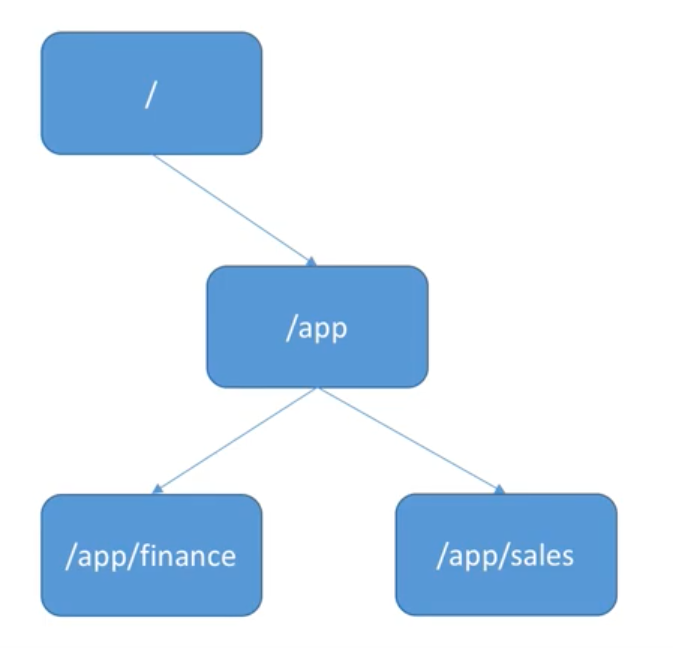
\includegraphics[scale=0.3]{images/zookeeper-node.png}
    \caption{ZooKeeper zNodes (02.04.2020)}
    \url{https://youtu.be/AS5a91DOmks?t=161}
    \label{img:}
\end{figure}
Die Eigenschaften einer zNode sind, dass jede über einen Pfad verfügt und entweder persistent oder ephermal sein kann - Kafka verwendet beide. Mit persistent ist gemeint, dass die zNode immer existiert, also somit eine persistente Präsenz aufweist. Die ephemeral zNode ist nur zur Zeit der Verbindung mit der Applikation existent. Darüber hinaus kann eine zNode Daten speichern, kann nicht umbenannt werden und bietet die Möglichkeit für eine Observierung. Heißt, dass sich Abonnenten dieser zNode darüber informieren lassen können, ob eine Änderung in dieser stattgefunden hat.
(vgl. \cite{ZooKeeper-Video})
\subsubsection{Entscheidungsprozess}
Als ein Bestandteil von Kafka, fällt eine jede direkte Entscheidung weg, da eine Entscheidung für Kafka immer auch eine für Zookeeper ist.

\subsection{Kotlin[EK]}
\begin{figure}[H]
    \centering
    
\includegraphics[scale=0.1]{images/kotlin-logo.png}
    \caption{Kotlin Logo (02.04.2020)}
    \url{https://upload.wikimedia.org/wikipedia/commons/thumb/7/74/Kotlin-logo.svg/1024px-Kotlin-logo.svg.png}
\end{figure}
\subsubsection{Allgemein}
Bei Kotlin handelt es sich um eine relativ neue Sprache, welche im Jahre 2011 von JetBrains ins Leben gerufen wurde. Als Open-Source Sprache ist diese nicht allein von JetBrains abhängig, seit Google sie im Jahre 2017 als die neue offizielle Sprache für Android über Java ernannt hat. Folgend stiegen auch sie bei der Entwicklung ein. Darüber hinaus, wie bei den meisten Open-Source Projekten, beteiligt sich auch die Community an der Entwicklung der Sprache. Ziel der Sprache ist die Multiplattform. Kotlin-Code ist damit nicht nur auf der JVM lauffähig, sondern auch Native und im Web. Gemeinsam bilden Google und JetBrains die Kotlin Foundation.
\subsubsection{Merkmale}
\begin{itemize}
  \item \textit{Kurz und prägnant.} Ein sogenanntes POJO mit Gettern, Settern und Standardfunktionen, wie „toString()“ können in einer Zeile geschrieben werden. Lamda-Expressions erlauben Operationen, wie zum Beispiel das Filtern einer Liste, ohne viel Boilerplate-Code. 
  \item  \textit{Typsicherheit und keine NullPointer-Exceptions.} Kotlin ist eine stark und statisch typisierte Programmiersprache. Eine Variable für den Compiler darf nicht den Wert null annehmen, außer dies wird explizit angegeben. Bei einer Typenprüfung wird die Variable automatisch gecastet und erlaubt somit den direkten Zugriff auf die typenspezifischen Felder, Eigenschaften und Funktionen.
  \item  \textit{Interoperabel.} Kotlin kann, je nach Target-Plattform, auf die existierenden Öko-systeme zugreifen. So kann in der JVM-Plattform die große Vielfalt an existierenden Libraries genutzt werden.
\end{itemize}
(vgl. \cite{Kotlin-Lang})
\subsubsection{Syntax}
Da in Kontext dieses Projekts Kotlin vor allem als Ersatz für Java eingesetzt wird, wird hier die Syntax im Vergleich zu Java erläutert. Dies heißt, das auf Unterschiede eingegangen wird, welche vor allem der Veranschaulichung der Argumentation für den Entscheidungsprozess dienen soll.
\begin{lstlisting}[caption={Kotlin-Hello-World}, language=Kotlin]
fun main() {
    println("Hello world!")
}
\end{lstlisting}
\vspace{4mm}\par
Wie auch in Java ist die Main-Funktion der Einstiegspunkt der Applikation. Bereits jetzt wird im Beispiel ersichtlich, dass mit deutlich weniger Zeilen das klassische Hello-World-Programm geschrieben werden kann. In Kotlin darf auf die in Java obligatorische Klasse verzichtet werden; Funktionen werden im Unterschied mit dem Kürzel „fun“ deklariert. Es entfallen auch die Einstiegsargumente, welche bei Bedarf jedoch angegeben und verwendet werden können. Es entfällt in den meistens Fällen auch das Semikolon „;“. 
Hier der gleiche Code in Java:
\begin{lstlisting}[caption={Java-Hello-World}, language=Kotlin]
class HelloWorld {
    public static void main(String[] args) {
        System.out.println("Hello, World!"); 
    }
}
\end{lstlisting}
\vspace{4mm}\par
Im Bereich der Variablen bietet Kotlin alle bereits bekannten Datentypen, auch gibt es die Möglichkeit spezielle Datentypen über Java-Libraries zu nutzen. Im Unterschied zu Java muss der Datentyp nicht zwingend angeben werden, wenn der Compiler dies aus dem Kontext lesen kann. Hier die Möglichkeiten eine Variable zu deklarieren:
\vspace{3mm}\par
\newpage 
\begin{lstlisting}[caption={Val \& Var}, language=Kotlin]
val a: Int = 1
val b = 2
val c: Int 
var d = 3
\end{lstlisting}
\vspace{4mm}\par
An erster Stelle der Deklaration gibt die Art der Variable an, dies kann val oder var  sein. Val definiert eine read-only Variable. Bei Var hingegen handelt es sich um ein Variable, welche jederzeit, konform nach ihrem Datentyp, neu zugeordnet werden kann. 
Beim Wert c können wir sehen, dass der Compiler zu dieser Zeit noch nicht wissen kann, um welchen Datentyp es sich handelt, aus diesem Grund muss dieser explizit angegeben werden.
Eine weitere Besonderheit von Kotlin ist, dass ein „if“ auch als Expression fungieren kann, dies sieht wie folgt aus:
\vspace{3mm}\par
\begin{lstlisting}[caption={if-Expression}, language=Kotlin]
c = if (a > b) a else b
\end{lstlisting}
\vspace{4mm}\par
Hiermit wird immer die größere Zahl von a und b auf c zugewiesen.
(vgl. \cite{Kotlin-Basic-Syntax})
\subsubsection{Entscheidungsprozess}
Die Möglichkeiten wären Java, Python und Kotlin gewesen. Kotlin wurde als Sprache gewählt, da vor allem die schnelle Entwicklung von den Eigenschaften, wie weniger Boilerplate und dem Wegfallen der Nullpointer-Exceptions, profitiert. Dies sind aber vor allem persönliche Präferenzen, welche auch mit anderen Sprachen hätten erreicht werden können. Schlagkräftiges Argument war die Interoperabilität mit Java, da die Firma auf einer großen Java-Codebase sitzt. Wissen von Java kann daher schnell in Kotlin angewandt werden. Die Kompaktheit des Codes in Kotlin und der Möglichkeit auf Java-Code und deren Libraries zurückzugreifen unterstützte die Wahl.

\newpage
\subsection{NoSql Datenbanken [AA]}
Folgende Informationen wurden aus nachstehender Quelle bezogen. (vgl. \cite{bigdata_nosql_2020})
\subsubsection{Allgemeine Beschreibung}
NoSQL steht für Not only SQL und beschreibt Datenbanksysteme, die einen nicht-relationalen Ansatz haben. Datenbanken, die diesem Modell zugrunde liegen, sind horizontal skalierbar und lassen sich für Big-Data-Anwendungen einsetzen. Da NoSQL, Not only SQL bedeutet kann man nicht grundsätzlich auf die Datenbanksprache SQL (Structured Query Language) verzichten. Viele dieser Systeme setzen zwar komplett auf nicht relationale Funktionen, doch existieren auch NoSQL Datenbanken, die nur bestimmte Elemente von SQL-Systemen unberücksichtigt lassen.\\

Während relationale Datenbanken Tabellen mit Zeilen und Spalten für die Datenspeicherung verwenden, nutzen NoSQL Datenbanken zum Beispiel Objekte, Dokumente, Liste etc. für die Organisation der Daten. Diese Systeme haben eines gemeinsam, dass sie optimiert sind für Aufgaben, bei denen SQL Systeme an ihre Grenzen stoßen.\\

Aufgrund des Aufbaus skalieren NoSQL-Datenbanken horizontal. In vielen Fällen sind dies Open Source Softwares, doch gibt es einige Ansätze, die auf eine kommerzielle Lösung basieren. Durch das Fehlen eines Schemas, sind NoSQL Systeme flexibel einsetzbar und eigenen sich für große Datenmengen, wie sie aus Big Data Anwendungen kommen. Die Architektur ist auf Skalierbarkeit und Performance ausgelegt. Fast alle NoSQL Ansätze und Modelle lassen sich in vier Hauptkategorien einteilen. Diese sind Key-Value Datenbanken. Dokumentenorientierte Datenbanken, Spartenorientierte Datenbanken und Graphen Datenbanken.\\

Folgende Eigenschaften zeichnen die NoSQL Systeme aus: das Vermeiden unnötiger Komplexität, eine hohe Performance, die horizontale Skalierbarkeit, die Vermeidung von relationalen Ansätzen des Datenmappings, die Unterstützung der aktuellen Hardwaregenerationen und die Einfachheit in der Installationen und Konfiguration von verteilten Clustern.
\newpage
\subsection{Dokumentenorientierte Datenbanken}
Für diese Informationen wurde auf folgende Quelle zurückgegriffen. (vgl. \cite{ionis_dokumentenorientierte_2020})
\subsubsection{Allgemein}
Dokumentorientierte Datenbanken oder auch Document Stores genannt, finden Verwendung in der Verwaltung von semistrukturierten Daten. Mit semistrukturierten Daten sind Daten gemeint, die keine feste Struktur haben, sondern die Struktur selbst aus den Daten hervorgeht. Durch die fehlende klare Struktur in den Daten sind diese nicht für relationale Datenbanken geeignet, da sich die Informationen nicht in Tabellen einordnen lassen.\\

Die Datenbank erstellt dann einen Schlüssel zu jedem Dokument damit alles zugeordnet ist. Im Dokument selbst, dass zum Beispiel mit JSON, YAML oder XML formatiert ist sind die eigentlichen Daten gespeichert. Da die Datenbank kein bestimmtes Schema hat, kann man auch verschiedene Dokumenttypen gemeinsam in eine Dokumentorientierte Datenbank einbinden. Änderungen der Daten in den Dokumenten müssen nicht der Datenbank mitgeteilt werden.\\
 
Daten unterschiedlichster Formate und ohne gemeinsames Schema können in ein Document Store untergebracht werden. In der Praxis wird in der Regel nur ein Dateiformat für die Dokumente verwendet. Anschließend wird durch die Informationen eine feste Struktur aufgebaut. Durch diese festgelegten Regeln ist es einfacher die Daten zu verarbeiten zusätzlich wird die Arbeit mit der Datenbank verleichtert. Aufgrund dieser Ordnung können Suchanfragen an die Datenbank viel besser verarbeitet werden. In einer dokumentbasierten Datenbank können die gleichen Aktionen durchgeführt werden wie auch in einer relationalen Datenbank. Daten lassen sich einfügen, löschen, abfragen und ändern.\\
 
Damit sich diese Aktionen durchführen lassen, erhält jedes einzelne Dokument einen eindeutigen Schlüssel. Wie dieser Schlüssel zusammengesetzt wird, ist im Grunde egal. Eine einfache Zeichenfolge, der komplette Pfad oder andere Methoden können genutzt werden um das Dokument zu adressieren.
\newpage
\subsubsection{Mongo DB}\label{ssec:MongoDB}
\begin{figure}
\centering
	
\includegraphics[scale=0.05]{images/MongoDB.png}
	\caption[MongoDB (01.04.2020)]{MongoDB (01.04.2020)}
	\url{https://cdn.worldvectorlogo.com/logos/mongodb.svg}
	\label{fig:sample}
\end{figure}
Als Grundlage nachstehender Informationen dienten folgende Quellen. (vgl. \cite{mongodb_beliebteste_2020} \& \cite{scale_cassandra_2020} \& \cite{jepsen_jepsen_2020})
\paragraph{Allgemein}\mbox{} \\	
„MongoDB ist eine universelle, dokumentbasierte, verteilte Datenbank für die moderne Anwendungsentwicklung und die Cloud, die in puncto Produktivität höchsten Ansprüchen gerecht wird.“~\cite{mongodb_beliebteste_2020}

\paragraph{Expressive Object Model}\mbox{} \\
MongoDB unterstützt ein ausdrucksstarkes Objekt Modell. Objekte in der MongoDB können Eigenschaften haben und in sich selbst verschachtelt sein. Ein Objekt kann also mehrere Stufen haben. Dieses Modell ist sehr objektorientiert und kann jede Objektstruktur leicht repräsentieren. Außerdem kann jedes Objekt indexiert werden, noch dazu auf jeder Stufe.
\paragraph{Sekundäre Indizes}\mbox{} \\
Dieses Konzept vereinfacht es jede Eigenschaft eines Objekts zu indexieren egal, ob es verschachtelt ist oder nicht. Dadurch wird es einfacher diese Indizes abzufragen und die Ergebnisse davon zu erhalten.
\paragraph{Hohe Erreichbarkeit}\mbox{} \\
Die Datenbank unterstützt ein Single Master Model. Das bedeutet, dass es einen Eltern Knoten und viele Kinder Knoten gibt. Falls der Eltern Knoten ausfällt oder einfach nicht mehr funktioniert wird ein Kind der neuen Eltern Knoten. Früher benötigte dieser Prozess, 10 bis 40 Sekunden, aber seit neuesten wird alles unter 2 Sekunden geregelt. Während der Zeit bis ein neuer Elternknoten gefunden wird, rennt das Replika Set nicht und nimmt keine Schreibbefehle an. \\
\newpage
\paragraph{Schreib Skalierbarkeit}\mbox{} \\
MongoDB kann mit seinem Single Master Model nur auf seinen Primären Server Schreibbefehle annehmen. Während die sekundären Server nur für Lesebefehle benutzt werden. Wenn die Datenbank drei Replika Sets hat kann nur der Eltern Knoten Schreibbefehle entgegennehmen, während die Kinder nur Lesebefehle ausführen können. Dies schränkt die Skalierbarkeit sehr ein. Hierfür können aber alle Knoten gestriped werden, damit jeder einzelne Knoten Lese- beziehungsweise Schreibbefehle entgegen nehmen kann.
\paragraph{Query Language Support}\mbox{} \\
Die Datenbank hat eine eigene Query Language, kann aber auch ANSI SQL unterstützen.
\paragraph{Benutzbarkeit}\mbox{} \\
MongoDB ist eine einfach zu benutzende Datenbank die auch leicht aufgesetzt wird. Da die Dokumente in der Datenbank fast wie im Code aussehen ist es oft leicht die Objekte zu verstehen und zu benutzen. Auch hat MongoDB eine Vielzahl an Treibern und Applikationen um die Datenbank zu warten und darauf zu arbeiten.
\paragraph{Native Aggregation}\mbox{} \\
Die Datenbank hat ein eingebautes Aggregierungs Framework um die Daten in der Datenbank für eine ETL Pipeline zu transformieren. Dieses Framework ist für kleine und mittelgroße Daten um Anfragen zu bearbeiten. Desto größer die Datenmenge desto komplizierter wird dieser Prozess zu debuggen. Um größere Anfragen zu debuggen wird daher öfter Spark \ref{ssec:Spark} und Hadoop benutzt. Dies sind Tools mit ihren eigenen Ressourcen, Skills und vielen anderen Faktoren.
\paragraph{Schema-less Model}\mbox{} \\
In MongoDB kann ausgewählt werden, ob ein Schema auf die Dokumente forciert wird oder nicht. Seit der Version 3.2 ist dies möglich. Jedes Dokument kann seine eigene Struktur haben und die Applikationen interpretieren dann selbst diese Daten korrekt. Für einige Applikationen ist diese Flexibilität nötig.

\paragraph{Latenzzeit}\mbox{} \\
Als Erstes wird in der Datenbank ein primärer Knoten ausgewählt und die Replika State Maschine aufgebaut. Es gibt kein äußerliches System, dass dem Replika Set sagt, was es zu tun hat. Das Set selbst sucht den primären Knoten aus, bestimmt wann es sich selbst replizieren soll, etc.\\

Zusammengefasst ist MongoDB nicht die beste Wahl für ein Data Warehouse, da es öfters zu Datenverluste kommt. Doch das geht stark gegen das Konzept von einem Datawarehouse. 
\newpage
\subsection{Wide-Column Datenbanken}
Für folgendenden Text wurde jene Quelle verwendet. (vgl. \cite{dbengines_wide_2020})
\subsubsection{Allgemein}
Wide Column Datenbanken, auch Wide Column Stores, Extensible Record Stores und zu deutsch splatenorientierte Datenbank, speichern die eingehenden Daten in Datensätzen mit potentiell sehr vielen dynamischen Spalten ab. Da nicht nur der Schlüssel der Datensätze fix ist, sondern auch der Splatenname, kann davon gesprochen werden, dass ein Wide Column Store auch als zweidimensionaler Key Value Store angesehen werden kann. Ähnlich zu Document Stores haben Wide Column Datenbanken auch die Eigenschaft der Schemafreiheit, doch setzen beide Modelle diese Eigenschaft sehr verschieden um.
\subsubsection{Cassandra}\label{ssec:Cassandra}
\begin{figure}[H]
\centering
  
\includegraphics[scale=0.15]{images/Cassandra.png}
  \caption[Cassandra (01.04.2020)]{Cassandra (01.04.2020)}
  \label{fig:Cassandra}
  \url{https://upload.wikimedia.org/wikipedia/commons/thumb/5/5e/Cassandra_logo.svg/1280px-Cassandra_logo.svg.png}
\end{figure}
Für die weiterführenden Informationen wurden diese Quellen eingesehen. (vgl. \cite{scale_cassandra_2020} \&  \cite{bigdata_grundlagen_2020} \& \cite{jepsen_cassandra_2020})
\paragraph{Allgemein}\mbox{} \\
„Cassandra zählt, neben MongoDB, zu den derzeit populärsten NoSQL-Datenbanken. Cassandra ist als skalierbares, ausfallsicheres System für den Umgang mit großen Datenmengen auf verteilten Systemen (Clustern) konzipiert. In drei Teilen erläutert BigData-Insider die architektonischen Merkmale von Cassandra, erklärt die Inbetriebnahme sowie grundlegende Prinzipien und illustriert erste Schritte mit der Abfragesprache Cassandra Query Language (CQL).“~\cite{bigdata_grundlagen_2020}
\newpage
\paragraph{Expressive Object Model}\mbox{} \\
Im Gegensatz zu MongoDB bietet Cassandra eine schönere Struktur der Daten durch Tabellen mit Spalten und Zeilen. Durch diese Ansicht sind die Daten besser strukturiert und jede Spalte hat genau einen spezifizierten Typen der bei der Erstellung angegeben wurde.
\paragraph{Sekundäre Indizes}\mbox{} \\
In Cassandra sind sekundäre Indizies nur auf einzelne Spalten limitiert und werden nur auf Gleichheit geprüft. In der Datenbank sollte immer nach dem primären Schlüssel gesucht werden.
\paragraph{Hohe Erreichbarkeit}\mbox{} \\
Cassandra unterstützt ein Multiple Master System. Wenn ein Knoten ausfällt, oder nicht mehr funktioniert, funktioniert der Cluster noch weiterhin. Durch dieses System wird eine 100\% Uptime für Schreibbefehle zur Verfügung gestellt. 
\paragraph{Schreib Skalierbarkeit}\mbox{} \\
Durch das Multiple Master Model kann Cassandra Schreibbefehle auf jeden Server entgegennehmen. Desto mehr Server in einem Cluster sind, desto besser ist die Schreib Skalierbarkeit.
\paragraph{Qurey Language Support}\mbox{} \\
Cassandra unterstützt CQL als Query Language. CQL ist sehr nahe zu SQL. Durch diese Ähnlichkeit ist für Data Analystinnen und Analysten einfacher, die sich mit SQL auskennen auf Cassandra zu arbeiten. Doch unterstützt CQL nicht alles was SQL zu bieten hat. Einige der Funktionen die nicht unterstützt werden sind der Join oder Or Clauses. 
\paragraph{Benutzbarkeit}\mbox{} \\
Über die letzten Jahre ist es um einiges leichter geworden, Cassandra zu benutzen. Da Cassandra nun auch CQL als primäres Interface benutzt, ist es für alle die SQL beherrschen auch um einiges leichter geworden.
\paragraph{Native Gruppierung}\mbox{} \\
Cassandra hat keine native ETL Pipeline. Für Cassandra wird oft Spark \ref{ssec:Spark} oder Hadoop als Analyse Tool benutzt.
\paragraph{Schema-less Model}\mbox{} \\
In Cassandra, wegen CQL muss jeder Spalte ein Datentyp bei der Kreation mitgegeben werden.
\paragraph{Latenzzeit}\mbox{} \\
Nicht nur DataStax sondern auch die Open-Source Community für Cassandra haben seit Jahren hart daran gearbeitet das Cassandra kein AP Speicherhaltungsproblem mehr hat und dies zeigt sich. Cassandra kann tausende Knoten Cluster rennen lassen und phänomenale Verdichtungen von Schreibbefehle entgegennehmen. Durch dieses Engagement von Entwicklern ist Cassandra ein guter AP Datastore, der sich sehr gut eignet um ein Datawarehouse zu sein. Außerdem eignet sich Cassandra noch einmal besser als Datawarehouse, da wenn der Eltern Knoten ausfällt, direkt ein neuer gefunden wird und es somit keinen Schreibverlust gibt.

\subsection{In-Memory Datenbanken}
Referenzinformationen für diesen Text ist folgende. (vgl. \cite{datenbanken_-memory-datenbank_2020})
\subsubsection{Allgemein}
Dieser Datenbanktyp ist ebenfalls eine Art der NoSQL Datenbanken. In Memory Datenbanken, die auch als IMDB oder Hauptspeicher Datenbanken bekannt sind, werden für besonders große Datenmengen eingesetzt. Diese Datenbanken werden dann eingesetzt, wenn relationale Datenbanken an ihre Grenzen stoßen. Die Daten werden im Hauptspeicher abgelegt und somit erreichen diese Datenbank wesentlich schnellere Antwortzeiten. Außerdem werden die Daten so im Systemspeicher in komprimierter, nicht relationaler Form gehalten.\\

Die In Memory Datenbank gehört zu den analytischen Datenbanken. Diese Datenbanken bieten nur lesende Zugriffe und werden meist für die Datenhaltung historischer Daten verwendet. Meist sind In Memory Datenbanken Teil eines Data Warehouses.
\newpage
\subsubsection{Redis}
\begin{figure}[H]
\centering
  
\includegraphics[scale=0.25]{images/Redis.png}
  \caption[Redis (01.04.2020)]{Redis (01.04.2020)}
  \label{fig:Redis}
  \url{https://upload.wikimedia.org/wikipedia/de/thumb/6/6b/Redis_Logo.svg/1200px-Redis_Logo.svg.png}
\end{figure}
Diese Informationen sind aus folgender Quelle bezogen worden.(vgl. \cite{amazon_redis_2020})
\paragraph{Allgemein}\mbox{} \\
„Redis steht für Remote Dictionary Server und ist ein schneller Opensource In-Memory-Schlüsselwert-Datenspeicher für die Verwendung als Datenbank, Cache, Message Broker und Warteschlange. Das Projekt entstand, als Salvatore Sanfilippo, der ursprüngliche Entwickler von Redis, versuchte, die Skalierbarkeit seines italienischen Start-ups zu verbessern. Redis bietet jetzt Reaktionszeiten von unter einer Millisekunde und kann so Millionen von Anforderungen für Echtzeitanwendungen in den Bereichen Gaming, Ad-Tech, Finanzdienstleistungen, Gesundheitswesen und IoT verarbeiten. Redis wird gerne eingesetzt für Caching, Sitzungsmanagement, Gaming, Bestenlisten, Echtzeitanalysen, Geodaten, Mitfahrgelegenheiten, Chat/Messaging, Media-Streaming und Pub/Sub-Apps.“~\cite{amazon_redis_2020}
\paragraph{Funktionalitäten}\mbox{} \\
Da Redis eine In Memory Datenbank ist, befinden sich die Daten nicht auf einer Festplatte oder SSD. Dadurch fallen die Zugriffe auf die Platte beziehungsweise den Datenträger weg. Deswegen sind die Daten innerhalb von Mikrosekunden zugänglich. Redis stellt vielseitige Datenstrukturen, hohe Verfügbarkeit, Geodaten, Lua Scripting, Transaktionen, On Disk Persistenz und Cluster-Unterstützung zur Verfügung. Redis kann so helfen Echtzeit Apps leichter zu realisieren.
\subsubsection{Vorteile von Redis}
\paragraph{In Memory Datenbank}\mbox{} \\
Ein Vorteil von Redis ist das die Daten im Hauptspeicher des Servers gehalten werden und nicht wie bei Cassandra oder MongoDB die meisten Daten auf Festplatten beziehungsweise SSDs gespeichert sind. Da die Daten in Redis im Hauptspeicher gespeichert werden, wird die Zeit für den Lesebefehl gespart und somit werden die Daten um einiges schneller erhalten. Deswegen kann Redis als Data Mart für ein Data Warehouse verwendet werden um die Daten kurz zu halten um schneller darauf zuzugreifen. 
\paragraph{Flexible Datenstrukuren}\mbox{} \\
Im Gegensatz zu anderen Key Value Datenbanken bietet Redis eine Vielzahl an Datenstrukturen um mehrere Datentypen in Redis zu speichern. Es gibt folgende Datentypen in Redis:
\begin{itemize}
\item Zeichenkette \mbox{} \\
Dies können Text oder Binärdaten mit einer Größe von bis zu 512 MB sein.
\item Listen \mbox{} \\
Listen sind zusammen gehängte Zeichenketten.
\item Sätze \mbox{} \\
Sätze sind mehrere unsortierte Zeichenketten, die sich mit anderen überschneiden, vereinen oder voneinander unterscheiden können.
\item Sortierte Sätze \mbox{} \\
Dies sind nach Wert aufgelistete Sätze.
\item Hashes \mbox{} \\
Hashes sind eine Datenstruktur die zum Speichern einer Liste mit Feldern und Werten dienen.
\item Bitmuster \mbox{} \\
Ist ein Datentyp, der Vorgänge auf Bitebene ermöglicht.
\item HyperLog Protokolle \mbox{} \\
Dies ist eine Datenstruktur die eindeutige Elemente in einem Datensatz schätzt.
\end{itemize}
\paragraph{Einfachheit und Benutzerfreundlichkeit}\mbox{} \\
Der Code wird in Redis vereinfacht indem es wenige Codezeilen benötigt um Daten zu speichern, um diese zu verwenden und darauf zugreifen zu können. Es gibt viele verschiedene Open Source Clients die Verwendet werden können. Beispiele für diese Clients sind Java, Python, PHP, C, C++, Javascript, Node.js, Ruby, R, Go und viele mehr.
\paragraph{Replikation und Beständigkeit}\mbox{} \\
Weil Redis eine primäre Replikaarchitektur verwendet, unterstützt es so eine asynchrone Replikation, bei der Daten auf mehreren Replikatserver repliziert werden können. Dadurch kann von einer verbesserten Leseleistung ausgeganngen werden. Redis unterstützt auch Zeitpunktsicherungen, dies ist eine Kopie eines Redis Datensatzes auf eine Festplatte.  
\paragraph{Hohe Verfügbarkeit und Skalierbarkeit}\mbox{} \\
Redis kann auf einem Primärknoten oder in einem Cluster laufen. So können hochverfügbare Lösungen erstellt werden, die konsistente Leistung und Zuverlässigkeit ermöglichen. Da der Cluster horizontal und vertikal skaliert werden kann, kann so der Cluster genau auf die Anforderung angepasst werden.
\paragraph{Erweiterbarkeit}\mbox{} \\
Da Redis ein Open Source Projekt ist untersteht es keiner Abhängigkeit von einem Anbieter oder Technologie. Deswegen kann Redis so gut auf einzelne Fälle erweitert werden.

\subsubsection{Aerospike}
\begin{figure}[H]
\centering
  
\includegraphics[scale=0.2]{images/Aerospike.png}
  \caption[Aerospike (01.04.2020)]{Aerospike (01.04.2020)}
  \label{fig:Aerospike}
  \url{https://download.logo.wine/logo/Aerospike_(database)/Aerospike_(database)-Logo.wine.png}
\end{figure}
Für den folgenden Text ist folgende Quelle bezogen worden. (vgl. \cite{computer_funktionen_2020})
\paragraph{Allgemein}\mbox{} \\
„Aerospike ist ein In-Memory NoSQL Datenbank-Management-System (DBMS) auf Open-Source-Basis. Das Schlüssel-Werte-Datenbanksystem wurde entwickelt, um in Echtzeit Big-Data-Anwendungen möglichst schnell Antworten zu liefern. Da Aerospike vorwiegend mit Daten im RAM arbeitet, bietet es sehr geringe Zugriffszeiten, die nach Herstellerangaben bei 99,9 Prozent der Anfragen unter fünf Millisekunden liegen“~\cite{computer_funktionen_2020}
\paragraph{Funktionalitäten}\mbox{} \\
Diese In Memory Datenbank bietet verschiedenste Abfragemöglichkeiten unter der Verwendung von sekundären Indizes oder benutzerdefinierten Funktionen, die auf dem Aerospike Datenbankserver laufen. Aerospike kann aber auch mit neuartigen, komplexen Datentypen umgehen. Ein Beispiel hierfür wären Listen oder Maps. Außerdem stellt Aerospike verschiedenste Analytics Funktionalitäten zur Verfügung. Die Funktionen von Aerospike können in drei Hauptkomponenten aufgeteilt werden:
\begin{itemize}
\item{Aerospike Database Server} \mbox{} \\
Dies ist die Hauptfunktion von Aerospike. Er fungiert als Datenbank Engine und ist auf mehrere Knoten aufgeteilt. Außerdem ist er für die Datenspeicherung zuständig, die auf den Arbeitsspeicher oder SSD erfolgen kann.
\item{Aerospike Smart Clients} \mbox{} \\
Die Smart Clients wurden in den verschiedensten Programmiersprachen entwickelt und erstellt und halten ständig den Kontakt zu dem Aerospike Cluster. Zudem muss sich der Entwickler nicht darum kümmern selbst den Cluster zu informieren ob ein neuer Knoten hinzugekommen ist oder nicht. Dies läuft alles automatisch von Aerospike aus ab.
\item{Aerospike Management Console} \mbox{} \\
Diese Konsole ist eine Webschnittstelle, damit der/die AdministratorIn den Aerospike Cluster verwalten kann.
\end{itemize}
Dazu kommt die Enterprise Edition von Aerospike mit drei zusätzlichen Features die nicht in der Communtity Edition enthalten sind. Diese wären:
\begin{itemize}
\item{Cross Datacenter Replikation} \mbox{} \\
Diese Funktion ermöglicht es einem Unternehmen, mehrere Aerospike Cluster miteindander zu synchronisieren. Normalerweise sind diese Cluster in verschiedenen Rechenzentren. Es gibt diese Funktion um sicher zu gehen, dass das Unternehmen weiterhin arbeiten kann.
\item{Fast Restart} \mbox{} \\
Mit Fast Restart ist es möglich schnell Cluster upgraden zu können. Einzelne Server werden hinaufgefahren, ohne das die Indexe von den Daten auf den SSDs neu erstellt werden müssen.
\item{Benutzer- und Rollenbasierte Sicherheit} \mbox{} \\
Es gibt Benutzern Lese-, Schreib- und adminstrative Kontrolle.
\end{itemize}
Ein weiterer Vorteil von Aerospike ist es, dass Entwickler nicht dazu verplichtet sind sich mit Sharding- und Replikationsanforderungen zu plagen, da Aerospike dies automatisch durchführt.
\newpage
\subsubsection{Tarantool}
\begin{figure}[H]
\centering
  
\includegraphics[scale=0.3]{images/tarantool.png}
  \caption[Tarantool (01.04.2020)]{Tarantool (01.04.2020)}
  \label{fig:Tarantool}
  \url{https://dbdb.io/media/logos/tarantool.png}
\end{figure}
Folgendes Unterkapitel wurde mit folgenden Quellen umgesetzt. \cite{tarantool_tarantool_2020}
\paragraph{Allgemein}\mbox{} \\
Tarantool ist eine leistungsstarke schnelle Datenplattform mit einer In Memory Datenbank und einem integrierten Anwendungsserver. 
\paragraph{Funktionalitäten}\mbox{} \\
Einige Vorteile von Tarantool sind:
\begin{itemize}
\item{In Memory Datenbank} \mbox{} \\
Tarantool ist eine In Memory Datenbank. Dadurch hat die Datenbank stehst eine hohe Performance, einen hohen Durchsatz und geringe Latenzzeit. 
\item{Application Server} \mbox{} \\
Durch den Applikations Server kann die hohe Performance gesichert werden. 
\item{Replication Tools} \mbox{} \\
Durch die Replikation erlaubt es Tarantool auf mehreren Instanzen von sich aus zu arbeiten. Diese Instanzen stammen von der selben Datenbank. Dies funktioniert weil jede Instanz mit den anderen in Verbindung steht und so alle Änderungen erfasst werden. 
\item{ANSI SQL Features} \mbox{} \\
Ein weiterer Vorteil von Tarantool ist es, dass SQL Befehle benutzt werden können während alle Vorteile von NoSQL bezogen werden.
\item{Write Ahead Logging} \mbox{} \\
Durch erstellen von solchen Log Dateien oder Snapshots kann es nicht passieren, dass die Daten verloren gehen können.
\end{itemize}
\newpage
\subsection{Spark [AA]}\label{ssec:Spark}
\begin{figure}[H]
\centering
  
\includegraphics[scale=0.3]{images/Apache_Spark.png}
  \caption[Spark (01.04.2020)]{Spark (01.04.2020)}
  \url{https://upload.wikimedia.org/wikipedia/commons/thumb/f/f3/Apache_Spark_logo.svg/1200px-Apache_Spark_logo.svg.png}
  \label{fig:Spark}
\end{figure}
Mit folgender Quelle wurde dieser Text realisiert. (vgl. \cite{data_spark_2020})
\subsubsection{Beschreibung}
Spark ist ein Framework, das unter Open Source Lizenz öffentlich verfügbar ist. Es ist ein Top Level Projekt der Apache Software Foundation und enstand ursprünglich aus einem Forschungsprojekt.
Außerdem ist Spark ein Allzweck Tool zur Datenverarbeitung, oder eine sogenannte Data Processing Engine. Data Scientiests und Engineers setzten Spark ein, um äußerst schnelle Datenabfragen auf große Datenmengen im Terabyte Bereich ausführen zu können.
Spark ist außerdem ähnlich zu Hadoop, dank Parallelisierung sehr leistungsfähig und umfangreich mit Bibliotheken (z.B. für Machine Learning) und Schnittstellen ausgestattet. Allerdings ist Spark nicht für jede Big Data Analytics Aufgabe die beste Lösung. 
\subsubsection{Besonderheit an Spark}
\begin{figure}[H]
\centering
  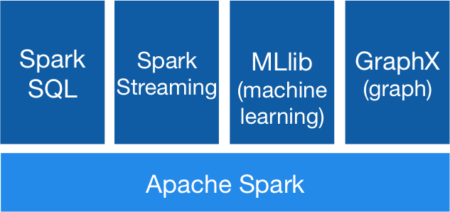
\includegraphics[scale=0.6]{images/spark.png}
  \caption[Spark Besonderheit (01.04.2020)]{Spark Besonderheit (01.04.2020)}
  \url{https://data-science-blog.com/wp-content/uploads/2016/08/spark-stack-1-1-450x212.png}
  \label{fig:Spark_Besonderheit} 
\end{figure}
Mit Spark können eingehende Daten transformiert, fusioniert und auch mathematisch analysiert werden. Typische Anwendungsszenarien von Spark sind interaktive Datenabfragen aus verteilten Datenbeständen und die Verarbeitung von fließenden Daten von Sensoren oder aus dem Finanzbereich oder auch andere. Die Stärke von Spark ist jedoch, dass Machine Learning eingebunden werden kann. Mit Zusätzen wie der Machine Learning Bibliothek (MLiB) oder SparkR (R Bibliotheken die direkt unter Spark verwendet werden). Im Unterschied zu Hadoop, das MapReduce Algorithmen benutzt, kann Spark sehr gut iterative Schleifen verarbeiten. Dies ist sehr wichtig für Machine Learning Algorithmen wie dem K Nearest Neighbour Algorithmus.\\

Seit der Entwicklung von Spark war es darauf ausgelegt, Daten dynamisch im RAM des Server Clusters zu halten und dort zu verarbeiten. Diese In Memory Technologien ermöglichen es besonders schnelle Auswertungen von Daten durchzuführen. Andere Datenbanken wie Redis oder SAP Hana arbeiten In Memory, doch kombiniert Spark diese Technik sehr gut mit der Parallelisierung von Arbeitsschritten über ein Cluster und setzt sich deutlich von anderen Datenbanken ab. Im Feld von Big Data werden aus Kostengründen noch oft mechanisch arbeitende Magnet Festplatten eingesetzt. Doch selbst mit zunehmender Verbreitung von sehr viel schnelleren SSD Festplatten, ist der Arbeitsspeicher hinsichtlich der Zeiten für Zugriff und Schreibbefehle von Daten unschlagbar. Einige Unternehmen berichten von einem hohen Geschwindigkeitsvorteil zu Hadoop.\\

Doch kann Spark nicht nur im Tera-, sondern auch im Petabyte Bereich analysieren. Große Cluster können aus tausenden physikalischen oder virtuellen Server bestehen und auch von Spark eingesetzt werden. Auch ist Spark ein echtes Big Data Framework. Ein Cluster skaliert mit seiner Größe linear in seiner Leistungsfähigkeit. Apache Spark bringt zudem auch sehr viele Bibliotheken und APIs mit, die mit den Programmiersprachen Java, Python, R und Scalar angesprochen werden können.\\

Diese sind ohne Zweifel die verbreitetsten Sprachen, wenn es um Data Science geht. Durch die Flexibilität und geringe Rüstzeit wird Spark in vielen Projekten eingesetzt. Zudem kann es eine große Herausforderung sein ein Data Science Team mit gleichen Programmiersprachen Skills aufzubauen. Durch die Nutzung mehrerer Programmiersprachen kann Spark dieses Problem teilweiße lösen, beziehungsweise kann es so umgangen werden. Durch die APIs, die Spark zur Verfügung stellt können auch Daten von vielen verschiedenen Systemen abgegriffen werden. Beispiele wären hier Cassandra \ref{ssec:Cassandra} oder MongoDB \ref{ssec:MongoDB}.
\subsubsection{Gängige Anwendungsbeispiele für Spark}
\paragraph{ETL Datenintegration}\mbox{} \\
Spark eignet sich sehr gut um Daten aus unterschiedlichsten Quellen zu filtern und diese zu bereinigen um sie letztendlich zusammenzuführen. 
\paragraph{Interaktive Analysen}\mbox{} \\
Außerdem eignet sich Spark aufgrund seines Abfrage Systems fantastisch um interaktive Analysen von großen Datenmengen durchzuführen. Es gibt typische Fragestellungen die aus dem Buisness Analytics kommen. Diese können beispielsweise lauten, welche Quartalszahl für bestimmte Vertriebsregionen vorliegt, oder wie hoch die Produktionskapazitäten sind. Hier muss der Data Analyst nur die richtige Frage stellen und Spark liefert die richtige Antwort. 
\paragraph{Echtzeit Analysen von Datenströmen}\mbox{} \\
Mit Spark werden heute noch Massen von Maschinen- beziehungsweise Finanzdaten im Sekundentakt ausgewertet. Für Spark ist dies ein gängiges Einsatzgebiet. Daten, die von vielen verschiedenen Systemen generiert werden, können mit Spark ohne Probleme in einer hohen Geschwindigkeit zusammengeführt und sogleich analysiert werden. Ein Beispiel aus der Finanzwelt wäre, dass Kredikarten Unternehmen Spark dazu benutzen um in naher Echtzeit auf potenzielle Kreditkartenmissbräuche zu bemerken. 
\paragraph{Machine Learning}\mbox{} \\
Durch die Fähigkeiten die Spark hat wird es oft von vielen als erste Wahl zu Machine Learning empfohlen. Dies ist der Fall, da Spark Daten iterativ im Speicher und parallel in einem Cluster durchlaufen kann.

\subsection{Python [AA]}
\begin{figure}[H]
\centering
  
\includegraphics[scale=0.75]{images/python.png}
  \caption[Python (01.04.2020)]{Python (01.04.2020)}
  \url{https://i.pinimg.com/originals/0f/60/19/0f6019e15f1d8ae07e7e8ea16d242676.png}
  \label{fig:Python}
\end{figure}
Folgendes Kapitel wurde mit der folgenden Quelle bewerkstelligt. (vgl. \cite{bigdata_python_2020})
\subsubsection{Allgemein}
„Python ist eine Programmiersprache, die dank ihrer klaren Syntax und einfachen Lesbarkeit leicht zu erlernen ist und sich sehr vielseitig einsetzen lässt. Für die gängigen Betriebssysteme ist Python frei verfügbar. Die üblichen Programmierparadigmen wie die objektorientierte oder funktionale Programmierung werden unterstützt.“~\cite{bigdata_python_2020}
\subsubsection{Zentrales Merkmal von Python}
Der Ruf von Python ist ein guter, da es eine einfache und saubere Programmiersprache ist die eine klare Struktur hat. Der Programmcode ist intuitiv benutzbar und gleichzeitig leicht lesbar. Obwohl Python einfach ist, kann es gut skalieren und ist auch für komplexe Softwareprojekte einsetzbar. Damit Python so einfach und übersichtlich ist, kommt es mit sehr wenigen Schlüsselwörter aus. Außerdem verwendet Python dazu Einrückungen als Strukturierungselemente.\\

Im Gegensatz zu anderen Sprachen sind verschiedene Programm Blöcke nicht durch bestimmte Schlüsselwörter oder Klammern markiert, sondern durch einfache Einrückungen im Code. Ein weiteres Merkmal von Python ist die automatische Speicherverwaltung. Durch die dynamische Typisierung ist es nicht notwendig, Typen von Variablen oder Funktionsargumente im Vorhinein zu definieren.\\

Ein weiterer Punkt ist, dass niemand in Python an einen bestimmten Programmierstil gebunden ist. So kann für jede Aufgabe der optimale Programmierstil gewählt werden. Zusätzlich ist es möglich verschiedenste Python Programme in andere Sprachen einzubetten.
\subsubsection{Vorteile von Python}
Python bietet eine Vielzahl von Vorteilen. Zum Beispiel ist ein großer Vorteil von Python, dass es durch die einfache Syntax eine einfach zu lernende Sprache ist. Der größte Vorteil ist, dass Python eine schnelle Programmiersprache ist die viele Data Analystinnen und Analysten oder Machine Learning Prozesse benutzen. Deswegen wird Python oft für den ETL Prozess oder für die Analyse verschiedenster Daten benutzt. Python ist außerdem eine Objektorientierte Sprache, die komplexe Datenstrukturen verwalten und verarbeiten kann. Die Flexibilität von Python ist ein Grund warum die Programmiersprache von Data Analystinnen und Analysten gemocht wird. Durch diese Vorteile ist es klar, dass Python oft für Data Analytics benutzt wird.
\subsubsection{Philosophie von Python}
Hier sind alle Grundsätze von Python aufgelistet. Die „Zen of Python":\\
„Beautiful is better than ugly. \\
Explicit is better than implicit. \\
Simple is better than complex. \\
Complex is better than complicated. \\
Flat is better than nested. \\
Sparse is better than dense. \\
Readability counts. \\
Special cases aren't special enough to break the rules. \\
Although practicality beats purity. \\
Errors should never pass silently. \\
Unless explicitly silenced. \\
In the face of ambiguity, refuse the temptation to guess. \\
There should be one-- and preferably only one --obvious way to do it. \\
Although that way may not be obvious at first unless you're Dutch. \\
Now is better than never. \\
Although never is often better than *right* now. \\
If the implementation is hard to explain, it's a bad idea. \\
If the implementation is easy to explain, it may be a good idea. \\
Namespaces are one honking great idea -- let's do more of those!" \cite{python_pep_2020}
\subsection{Pyspark [AA]}
\begin{figure}[H]
\centering
  
\includegraphics[scale=0.7]{images/pyspark.png}
  \caption[Pyspark (01.04.2020)]{Pyspark (01.04.2020)}
  \url{https://i.pinimg.com/originals/97/e2/e1/97e2e161dafc63a9e98e5f350425ba39.png}
  \label{fig:Pyspark}
\end{figure}
Informationen wurden von der folgenden Quelle übernommen und überarbeitet. (vgl. \cite{says_pyspark_2020})
\subsubsection{Allgemein}
PySpark ist eine Python API die es ermöglicht Spark und Python zu verbinden. Diese Erweiterung wurde von der Apache Spark Community entwickelt und veröffentlich um Python in Spark zu benutzen. Wenn PySpark benutzt wird, kann leicht mit Resilient Distributed Databases gearbeitet und diese integriert werden. Außerdem gibt es eine Anzahl von Funktionen die Pyspark gut mit großen Datensätzen arbeiten lässt. Sei es eine Funktion auf die Daten auszuführen oder diese zu analysieren.
\subsubsection{Hauptfunktionen von Pyspark}
\begin{itemize}
\item{Real time computations} \mbox{} \\
Da Pyspark auf In Memory Technologien zurückgreift, zeigt sich eine geringe Latenzzeit.
\item{Polyglot} \mbox{} \\
Pyspark kann auch mit anderen Sprachen wie Scala, Java, Python oder R benutzt werden. Dadurch ist es ein oft genutztes Framework das verwendet wird um große Datenmengen zu analysieren.
\item{Caching and Disk Persistence} \mbox{} \\
Es bietet ein gutes Caching und eine gute Persistenz der Daten.
\item{Fast processing} \mbox{} \\
Ein weiterer Vorteil ist, dass PySpark um einiges schneller ist als andere Frameworks die mit Big Data arbeiten. 
\item{Works well with RDDs} \mbox{} \\
Da Python dynamisch ist, hat es den Vorteil, wenn es mit RDDs arbeitet.
\end{itemize}
\subsubsection{Nutzen von Pyspark}
Python ist eine verbreitete Sprache bei Data Scientists und Data Analystinnen und Analysten. Auf der anderen Hand ist Spark ein starkes Tool um mit Big Data umzugehen. Deswegen hat die Spark Community, PySpark entwickelt um beide zu verbinden.




\subsection{Docker [FK]}
\begin{figure}[H]
    \centering
    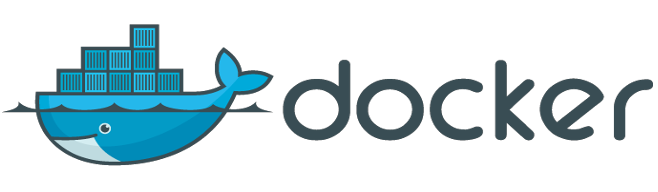
\includegraphics[scale=.67]{images/DockerLogo.png}
    \caption{Docker (01.04.2020)}
    \url{https://www.netways.de/wp-content/uploads/2016/02/DockerLogo.png}
\end{figure}
Docker ist eine Open-Source Plattform für das Ausliefern von Softwareprodukten. Mit Docker kann man die verschiedenen Teile eines Softwareproduktes wie Datenbanken, Server und Clients in einzelne Umgebungen verteilen, sogenannte Container [\ref{ssec:DockerContainer}]. Somit kann jede Komponente einzeln gestartet, konfiguriert, überwacht und getestet werden. Durch diese Modularität können Container fast unabhängig vom Betriebssystem arbeiten. (vgl. \cite{DockerIntro})
\subsubsection{Container} \label{ssec:DockerContainer}
\begin{figure}[H]
    \centering
    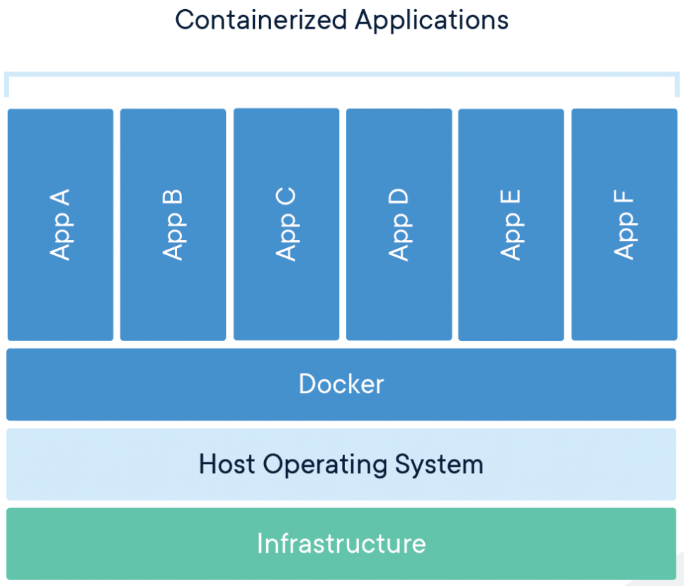
\includegraphics{images/what-is-a-container.png}
    \caption{Docker Container Architektur (01.04.2020)}
    \url{https://www.docker.com/sites/default/files/d8/styles/large/public/2018-11/container-what-is-container.png?itok=vle7kjDj}
    \label{img:what-is-a-container}
\end{figure}

Ein Container ist wie bereits in der Einleitung beschrieben ein abgeschlossenes Objekt welches mit einem oder mehreren Images (\ref{ssec:DockerImages}) als Bauplan erzeugt wird und alle nötigen Dinge beinhaltet was die Software zum Laufen braucht wie die Runtime, Libraries, Einstellungen und natürlich der Code der Applikation. Wie in der Grafik (\ref {img:what-is-a-container}) beschrieben liegen die einzelnen Container auf der Docker Engine auf welche die Container verwaltet und die nötigen Ressourcen vom Betriebssystem zu Verfügung stellt. Dadurch wird sichergestellt das der Code so isoliert von der Umgebung ist wie möglich. (vgl. \cite{DockerContainer})
\subsubsection{Images} \label{ssec:DockerImages}
Ein Docker Image besteht aus mehreren Schichten welche zur Ausführung von Code in einem Docker-Container verwendet wird. Ein Image wird im Wesentlichen aus den Anweisungen für eine vollständige und ausführbare Version einer Anwendung erstellt, die sich auf dem Kernel des Host-Betriebssystems stützt. (vgl. \cite{DockerImage})
Images sind extrem leichtgewichtig, weil sie auf das notwendigste reduziert sind und sicher da diese standardmäßig nicht von anderen Containern beeinflusst werden können. Ein gutes Beispiel dafür ist das Alpine Linux siehe Abbildung (\ref{img:docker-image-size}). Um dennoch mit anderen Containern und anderen Dingen wie dem File System interagieren zu können gibt es sogenannte Networks (\ref{ssec:DockerNetworks}).
\begin{figure}[H]
    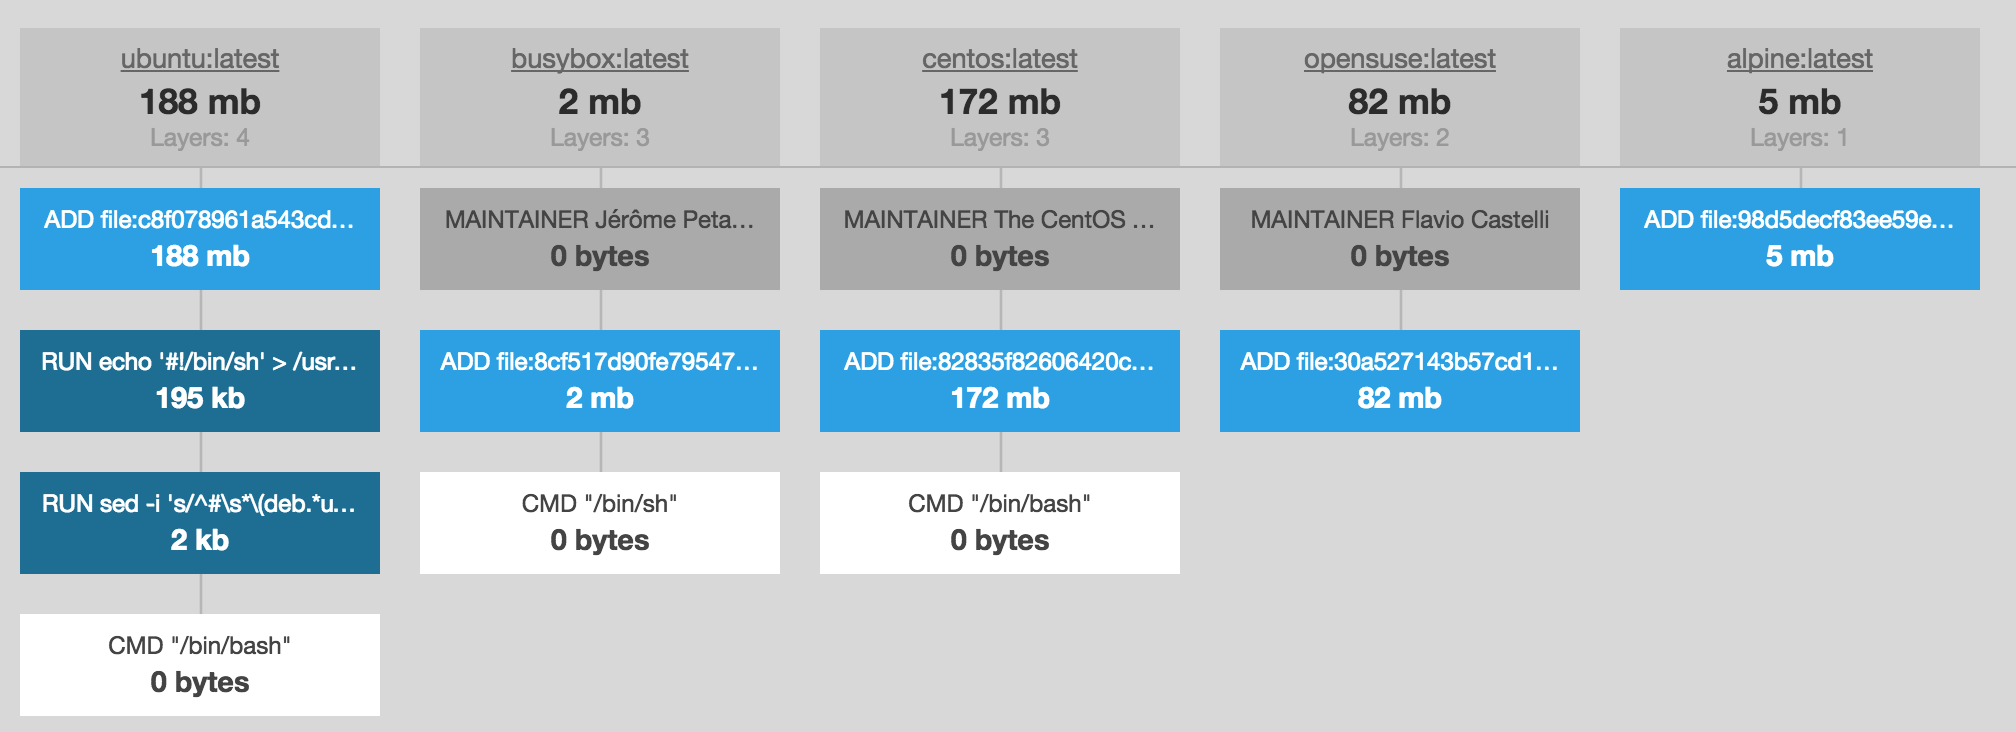
\includegraphics[scale=.40]{images/Docker_Image_Size.png}
    \caption{Docker Image größenvergleich (01.04.2020)}
    \url{https://brianchristner.io/content/images/2015/07/Docker_Image_Size.png}
    \label{img:docker-image-size}
\end{figure}
\subsubsection{Networks} \label{ssec:DockerNetworks}
Networks(Netzwerke) verbinden die einzelnen Container miteinander. Es ist außerdem egal ob die Docker-Hosts unter Windows, Linux oder einer Mischung von beiden laufen. Die Networks verbinden beides Plattform unabhängig.Networks besitzen auch Möglichkeiten Docker unabhängige Systeme zu beeinflussen. Die verschiedenen Network Einstellungen werden im Kapitel Dockerfile [\ref{ssec:Dockerfile}] noch genauer Beleuchtet. (vgl. \cite{DockerNetworks})
\paragraph{Docker Produkte:}\mbox{}\\
\begin{itemize}
    \item Docker Toolbox [\ref{ssec:DockerToolbox}]
    \item Docker CE [Community Edition) (\ref{ssec:DockerCE}]
    \item Docker EE [Enterprise Edition) (\ref{ssec:DockerEE}]
    \item Docker Hub [\ref{ssec:DockerHub}]
    \item Docker Desktop [\ref{ssec:DockerDesktop}]
    \item Orchestration anhand von Kubernetes (\ref{ssec:DockerOrchestration}]
    \item Dockerfile [\ref{ssec:Dockerfile}]
    \item Docker-compose [\ref{ssec:Docker-Compose}]
\end{itemize}
\subsubsection{Docker Toolbox} \label{ssec:DockerToolbox}
Docker Toolbox ist eine veraltete Version von Docker. Es ist dennoch wichtig, weil ältere Betriebssysteme (Bsp. Windows 8) dennoch Docker installieren und verwenden können. Jedoch geht der große Vorteil von Docker verloren, weil anstatt der Docker Engine alles auf einer VirtualBox aufbaut. Somit geht einiges an Performance verloren, was aber beim Entwickeln kein Hindernis darstellt. Ein weiterer Use-Case der Docker Toolbox ist das verwenden auf PCs mit Windows 10 Home denn in der Home Version wird Hyper-V [\ref{Hyper-V}] nicht unterstützt. (vgl. \cite{DockerToolbox})
\subsubsection{Docker CE (Community Edition) / Docker Engine}\label{ssec:DockerCE}
Docker Community ist die klassische Open Source Version von Docker. Früher genannt Docker Engine. Alle oben genannten Funktionen sind ganz normal vorhanden ohne Kürzungen oder Ähnliches. Der geschriebene Sourcecode ist ebenfalls derselbe wie bei der Enterprise-Edition, weil beides auf dem Open Source Code von Docker aufbauen. Es gibt eine Stabile und eine experimentelle Version, bei welcher die neuesten Funktionen vorhanden sind, es aber noch immer Sicherheitslücken und Fehler geben kann. Vierteljährlich kommt eine neue Stabile Version heraus und jeden Monat gibt es eine neue experimentelle Version. (vgl. \cite{DockerCE})
\subsubsection{Docker EE (Enterprise Edition)}\label{ssec:DockerEE}
Docker Enterprise ist dafür da das Unternehmen ihre Container einfacher verwalten, starten und sichern können. Dabei gibt es drei verschiedene Versionen: Basic, Standard und Advanced.
\begin{itemize}
    \item Basic
    \begin{itemize}
        \item Spezielle Enterprise Betriebssysteme wie Windows Server oder Red Hat Enterprise Linux können verwendet werden.
        \item „same day“ Docker Support.
        \item Zertifizierte Container und Plugins aus dem Docker Hub.
    \end{itemize}
    \item Standard (Aufbauend auf Basic)
    \begin{itemize}
        \item Erweiterte Container- und Imageverwaltung.
        \item LDAP/AD Benutzer Integration. (\ref{sec:AD})
        \item Rollen basierte Zugriffskontrolle.
    \end{itemize}
    \item Advanced (Aufbauend auf Standard).
    \begin{itemize}
        \item Docker Security Scanning überprüft ob Images und Container frei von bekannten Sicherheitslücken sind.
        \item Kontinuierliche Überwachung von Schwachstellen.
    \end{itemize}
\end{itemize}
Wie bereits bei Docker Community angesprochen gibt es keine Unterschiede in der Funktionsweise der Docker Engine. Was jedoch auch bedeutet das man für seine 750\$ pro Prozessor pro Jahr für die Basic, 1500\$ für die Standard oder 2000\$ für die Advanced Version für Linux(Windows ist billiger) kein besseres Produkt bekommt, sondern nur oben genannte Boni. (vgl. \cite{DockerEE}, \cite{DockerEELicensing}, \cite{DockerEEPricing})
\subsubsection{Docker Hub} \label{ssec:DockerHub}
Docker Hub ist eine Website zur Verfügung gestellt von Docker wo User auf der ganzen Welt ihre Container Images hochladen können und sie somit mit anderen Usern teilen können. Man muss dabei nicht immer auf fragwürdige Quellen vertrauen, denn es gibt sogenannte „Official Images“ welche von Docker selbst veröffentlicht wurden und außerdem verifizierte und zertifizierte Veröffentlicher um auf der sicheren Seite zu sein das keine Malware im Image steckt. Das Container Image rauf- und runterladen ist dabei meistens gratis, jedoch muss man für die Erstellung von mehr als einem privaten Repository einer monatlichen Zahlung zustimmen. (vgl. \cite{DockerHub})
\subsubsection{Docker Desktop}\label{ssec:DockerDesktop}
Docker Desktop ist, wer hätte es gedacht, eine Desktop App für Windows und Mac OS. Der Download von Docker Desktop lädt automatisch alle benötigten Dateien, um die Community Version von Docker zu verwenden. Leider bedeutet das auch das Nutzer mit Windows 10 Home oder niedrigere Versionen von Windows dieses Tool nicht verwenden können und sich mit der CLI-Only (Command Line Interface Only) Version der Docker Toolbox zufriedengeben müssen. Sollte man aber Windows 10 Pro oder Enterprise besitzen, hat man mit Docker Desktop die Möglichkeit im Dashboard alle laufenden Container inklusive Kubernetes zu verwalten. Mit einem einzigen Klick kann man den Container somit kinderleicht Starten, Stoppen, Neustarten, den Port ändern oder direkt per Command Line darauf zugreifen. Außerdem kann man die Logs, die Image Einstellungen und diverse Statistiken betrachten. (vgl. \cite{DockerDesktopDashboard}, \cite{DockerDesktop}) 
\begin{figure}[H]
    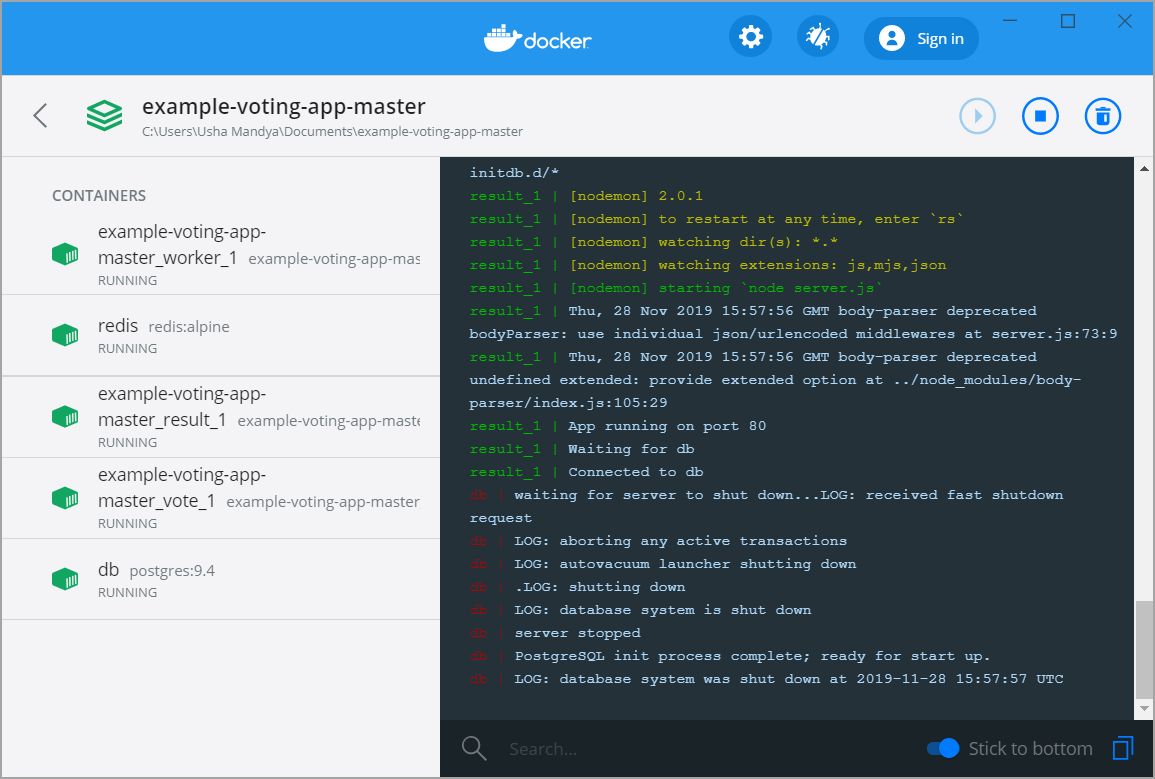
\includegraphics[scale=.65]{images/docker-desktop-view1.png}
    \caption{Docker Desktop Dashboard mit CLI (01.04.2020)}
    \url{https://docs.docker.com/docker-for-windows/images/application-view.png}
    \label{img:docker-desktop-view1}
\end{figure}
\begin{figure}[H]
    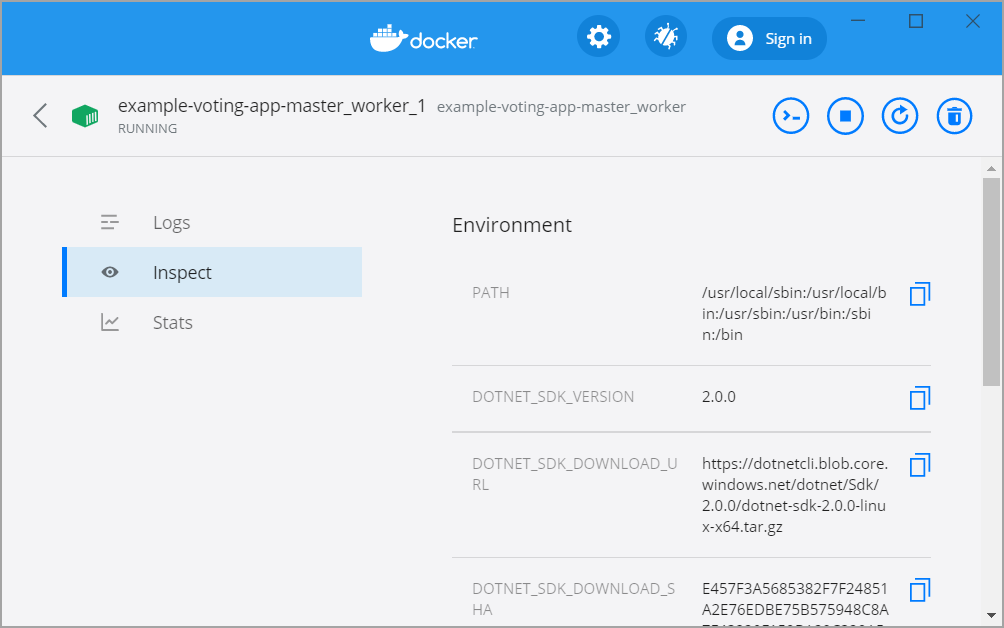
\includegraphics[scale=.70]{images/docker-desktop-view2.png}
    \caption{Docker Desktop Dashboard mit Monitoring (01.04.2020)}
    \url{https://docs.docker.com/docker-for-windows/images/container-view.png}
    \label{img:docker-desktop-view2}
\end{figure}
\subsubsection{Orchestration (with Kubernetes)}\label{ssec:DockerOrchestration}
\begin{figure}[H]
    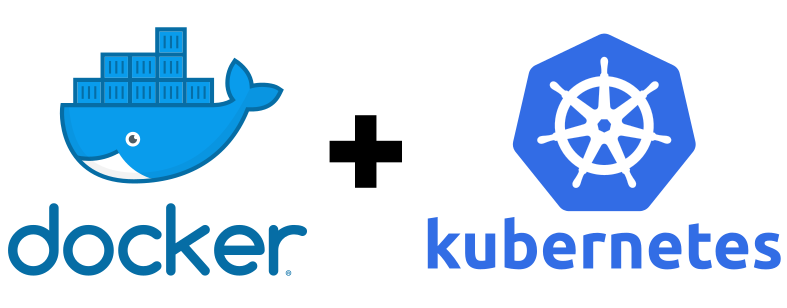
\includegraphics[scale=.50]{images/kubernetesLogo.png}
    \caption{Docker mit Kubernetes (01.04.2020)}
    \url{https://miro.medium.com/max/787/1*y320p_dXJmr5PMGRiXioyw.png}
\end{figure}
\paragraph{Was ist Orchestration und wofür wird sie benötigt}\mbox{}\\
Von Orchestration ist die Rede, wenn automatisiert viele verschiedene Computer zusammenarbeiten, um eine möglichst hohe Leistung und/oder hohe Verfügbarkeit zu erzeugen. Durch diese vielen verschiedenen Systeme und Programme steigt der Aufwand exponentiell mit der Anzahl der sogenannten Knotenpunkte(nodes). Dieser Aufwand kann eigenhändig ab einem gewissen Punkt nicht mehr bewältigt werden. Die Lösung: Automatisierung. Der Feine unterschied zwischen Automatisierung und Orchestrierung ist das die Orchestrierung auf der Automatisierung aufbaut. Eine einzelne Aufgabe kann Automatisiert werden aber wenn viele automatisierte Aufgaben zusammengeschlossen werden nennt man die Orchestrierung. 
\paragraph{Kubernetes und Docker}\mbox{}\\
Kubernetes wurde von Google entwickelt und 2014 als Open Source veröffentlicht. Kubernetes ermöglicht viele verschiedene Container zu verbinden, ohne dass man sich ständig Gedanken machen muss wie die Container untereinander kommunizieren, in welcher Reihenfolge die Container gestartet werden müssen oder was bei Programmabstürzen passiert. (vgl. \cite{DockerOrchestration})
\paragraph{Vorteile von Kubernetes}\mbox{}\\
\begin{itemize}
	\item Sollte ein Container abstürzen oder die Maschine defekt sein kann ein neuer Container auf einer anderen Maschine automatisch gestartet werden.
	\item Die Belastung der Container wird auf verschiedene Maschinen aufgeteilt.
	\item Es können verschiedene Instanzen eines Containers existieren wie z.b. bei einer Datenbank. Somit können kosten für die Anschaffung von extrem viel Speicher auf einer Maschine gespart werden.
	\item Wenn sich die Auslastung eines Containers verändert können Instanzen hinzugefügt oder weggegeben werden.
	\item Derselbe Code kann auf mehreren Maschinen gleichzeitig laufen
\end{itemize}
(vgl. \cite{DockerKubernetes})
\subsubsection{Das Dockerfile}\label{ssec:Dockerfile}
Das Dockerfile enthält die Logik, um ein Image aufzubauen. Das Dockerfile ist ein Text Dokument, welches die ganzen Kommandos enthält, die auch ein User auf der CMD [\ref{sec:CMD}] selber ausführen könnte. Der große Vorteil dabei ist das mit einem einzigen „docker build“ alle Kommandos automatisch ausgeführt werden. (vgl. \cite{Dockerfile})
\begin{figure}[H]
    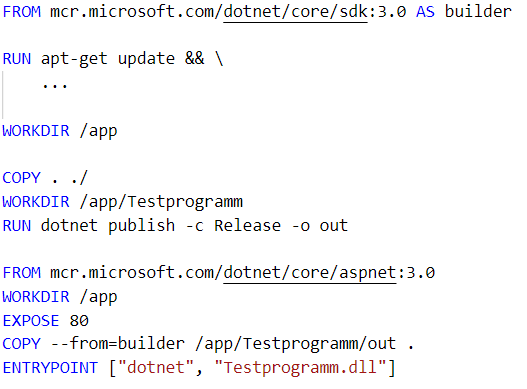
\includegraphics{images/dockerfile_example.PNG}
    \caption{Allgemeines Dockerfile Beispiel}
    \label{img:dockerfile_example}
\end{figure}
So könnte ein gesamtes Dockerfile aussehen.
Nun werden die einzelnen Teile erklärt:
\paragraph{Das FROM statement}\mbox{}\\
Mit dem FROM Statement kann ein bereits existierendes Image verwendet werden und auf dessen Basis weitergearbeitet werden. In diesem Fall wird das FROM genutzt, um eine dotnet core 3.0 sdk (Eine C\# Applikation) mit allem was es benötigt zu verwenden. Sollten mehrere FROM Statements in einem Dockerfile sein teilt FROM in mehrere Umgebungen. Nachdem in unserem Beispiel später noch ein FROM Statement steht, müssen wir das erste FROM Statement mit „AS build“ benennen, um es in dem COPY Befehl am Schluss wiederverwenden zu können. 
\paragraph{Das RUN Statement}\mbox{}\\
Mit dem RUN Statement können Befehle wie in der Command Line ausgeführt werden. Hier werden noch einige Linux Funktionen nach installiert. Allgemein kann aber alles Mögliche ausgeführt werden
\paragraph{Das WORKDIR Statement}\mbox{}\\
Das WORKDIR Statement setzt einfach das Verzeichnis zu dem eingegebenen. Wenn das Verzeichnis nicht existiert wird es erstellt.
\paragraph{Das COPY Statement}\mbox{}\\
Das COPY Statement kopiert einfach die Files von einem Ort zum anderen. Äquivalent zu „RUN cp …“
\paragraph{Das EXPOSE Statement}\mbox{}\\
Das EXPOSE Statement öffnet den Port der als Parameter mitgegeben wird. Beachte: der Port wird nur in dem Container geöffnet
\paragraph{Das ENTRYPOINT Statement}\mbox{}\\
Das ENTRYPOINT Statement fungiert als ein Aufruf eines Kommandos. Der erste Parameter zeigt das Kommando, das ausgeführt werden soll und danach können so viele Parameter folgen wie man braucht. In diesem Beispiel wird der Befehl "dotnet" aufgerufen und als Parameter bekommt der Befehl "Testprogramm.dll" mit
\subsubsection{Das Docker-Compose}\label{ssec:Docker-Compose}
Das Docker-Compose ist ein File in welchem mehrere Docker Container in der gewünschten Reihenfolge und Parametern automatisch aufgerufen werden können. Somit muss man nicht jeden Container und jedes Netzwerk einzeln per Hand aufrufen, sondern muss nur den Befehl: „docker-compose up“ ausführen und man hat sofort alle Container gestartet. Dadurch verringert sich nicht nur der Aufwand enorm, sondern auch die Fehler Quote, wenn man z.B. die Container nicht in der richtigen Reihenfolge oder mit den falschen Parametern startet.
Ein docker-compose kann entweder ein .yml oder .yaml File sein. Es ist jedoch immer wichtig die Einrückungen richtig zu setzen, weil es keine geschwungenen Klammern oder Ähnliches gibt wie in anderen Programmiersprachen. Allgemein ist es ähnlich zu dem oben genannten Dockerfile, weil wieder mit Statements beschrieben wird, was gemacht werden soll. 
\begin{figure}[H]
    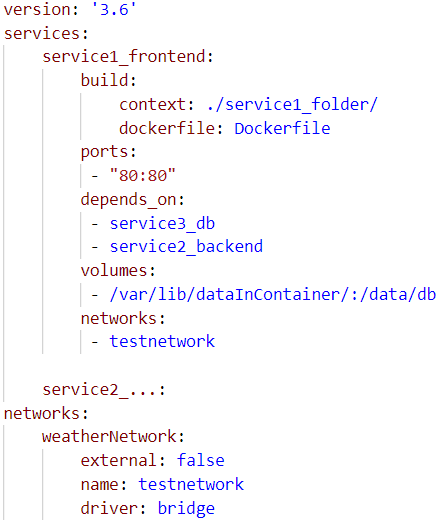
\includegraphics{images/docker-compose_example.PNG}
    \caption{Einfaches docker-compose Beispiel}
    \label{img:docker-compose_example}
\end{figure}
\subsubsection{Das Version Statement}
Das allererste in einem docker-compose ist das Version Statement. Damit wird dem Interpreter gesagt in welcher Version das folgende File geschrieben ist.
\subsubsection{Das Services Statement}
Das Services Statement beinhaltet alle Container, die gestartet werden sollen. Jedes Service bekommt einen Namen und den Pfad, wo das zugehörige Dockerfile liegt. Existiert bereits online ein fertiges Image, kann darauf verwiesen werden. Mit „ports“ kann man die offenen Ports festlegen. Rechts vom Doppelpunkt steht dabei der geöffnete TCP Port im Container und dieser wird auf den Docker Host Links vom Doppelpunkt gemapped. Bsp.: 8080:80 wenn man nun auf Port 8080 des Servers zugreift wird auf den Container am Port 80 weitergeleitet. Im nächsten Schritt wird festgelegt welche Services zuerst gestartet werden sollen. Im Bereich "volumes" kann eine Schnittstelle zu dem Host System geöffnet werden, um Daten permanent zu speichern welche sonst durch das neu erstellen des Containers verloren gehen würden. Mit dem Networks Bereich kann das Netzwerk ausgewählt werden, zu welchem das jeweilige Service gehört.
\subsubsection{Das Networks Statement}
Mit dem Networks Statement können ein oder mehrere Netzwerke erstellt werden. Wenn man das Netzwerk als extern deklariert kann man auf ein bereits existierendes Netzwerk von z.b. einem anderen docker-compose zugreifen. Außerdem kann man dem Netzwerk einen eigenen IP Adressraum geben. Das Networks Statement wird immer vor den Services aufgerufen.



\subsection{REST API [FK]} \label{sec:REST} 
Anmerkung: Folgendes wurde auf Basis von diesen Quellen geschrieben: (vgl. \cite{RestApi}, \cite{RestKonzept})
Rest bedeutet Representational State Transfer. API bedeutet Application Programming Interface.
Rest ist eine Möglichkeit über das Internet Daten zwischen verteilten Systemen auszutauschen. Es ist aber weder ein neues Protokoll noch Standard, sondern zeichnet jene Verfahren aus welche über das http Protokoll Daten versenden. Die versendeten Daten müssen aber nicht ein http Dokument sein denn das würde viel zu viele Stylings mitsenden, welche ungenutzt wären. Statt http wird JSON [\ref{sec:json}] oder XML [\ref{sec:xml}] verwendet. Diese beiden Formate können ausschließlich die Rohdaten enthalten und sind somit optimal. 
\begin{figure}[H]
    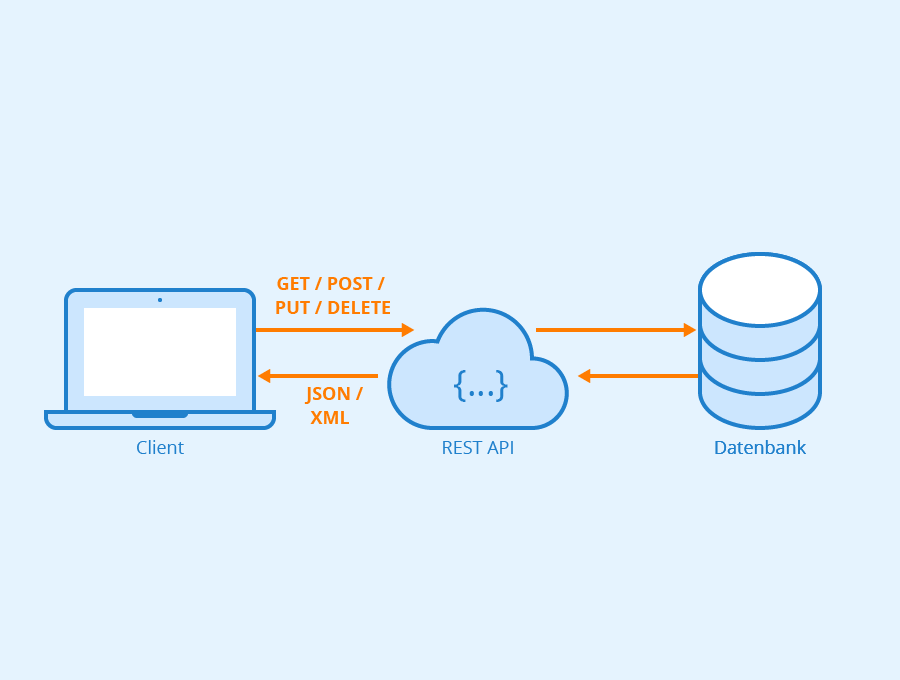
\includegraphics[scale=.9]{images/Rest-API.png}
    \caption{Rest Darstellung (01.04.2020)}
    \url{https://www.seobility.net/de/wiki/images/f/f1/Rest-API.png}
    \label{img:Rest}
\end{figure}
Wie bereits auf der Grafik zu sehen gibt es Grundsätzlich 4 verschiedene REST Requests. 
\subsubsection{GET Requests}
Mit dem GET Schlüsselwort wird dem empfangenen Server angezeigt das der Sender Daten haben will. Als Rückgabewert gibt es einen Return Code der bei Erfolg 200 (OK) lautet und bei Fehlschlag entweder 404 (Not Found) oder 400 (Bad Request). Außerdem wird bei Erfolg ein Body mit den Daten als JSON oder XML zurückgegeben.
Ein Typischer GET Request in cURL auf der Konsole würde so aussehen:
\begin{lstlisting}
    curl https://popularsite.com/getAllItems
\end{lstlisting}
\subsubsection{POST Requests}
Mit dem POST Request können Daten welche im Empfänger noch nicht existieren versendet werden. Bei Erfolg wird 201 (Created) zurückgegeben.
\subsubsection{PUT Requests}
Mit dem PUT Request können auch Daten erstellt werden aber hauptsächlich wird er dafür verwendet bestehende Datensätze zu Updaten. Wenn man sich aber nicht sicher ist ob der Datensatz (zum Beispiel ein Kunde) bereits existiert kann PUT verwendet werden um den Kunden neu hinzuzufügen sollte er noch nicht existieren ansonsten wird der Bestehende bearbeitet.
\subsubsection{DELETE Requests}
Mit dem DELETE Request können Daten auf dem Server gelöscht werden. 
\subsection{Die Architekturprinzipien von REST}
\subsubsection{Zustandslosigkeit}
Alle REST anfragen arbeiten „stateless“. Das bedeutet das in jedem Request alle Infos enthalten sein müssen damit der Empfänger genau weiß was zu tun ist. Nach jedem Request hat der Empfänger keine Informationen mehr wer ihm daten Geschickt hat oder woher. Somit erhöht sich die Skalierbarkeit und die Zuverlässigkeit, weil der Server nicht ständig eine Verbindung halten muss wie zum Beispiel bei einer Websocket Verbindung. Der Nachteil ist dabei eine Höhere Netzwerkauslastung 
\subsubsection{Caching}
Clients können die Antworten vom Server speichern umso die Netzwerkauslastung zu reduzieren. Der Nachteil dabei ist jedoch auf veraltete Daten zuzugreifen.
\subsubsection{Client-Server Modell}
Um Server besser Skalieren zu lassen muss der Client vom Server getrennt sein. Dies hat außerdem den Vorteil das der Client auf verschiedenen Plattformen ausführbar ist.
\subsubsection{Gleichartige Schnittstellen}
Alle REST Services nutzen das gleiche entkoppelte Interface. Somit wird sichergestellt das alles so einfach und einheitlich wie möglich ist. Der Nachteil dabei ist das nicht auf spezielle Anforderungen eingegangen werden kann.
\subsubsection{Hierarchisches System}
REST ist in mehreren Schichten aufgebaut wie folgende Grafik zeigt [\ref{img:Rest_Schichtenmodell}]. Jede Schicht kann aber nur die Anliegende „sehen“. 
\begin{figure}[H]
    \centering
    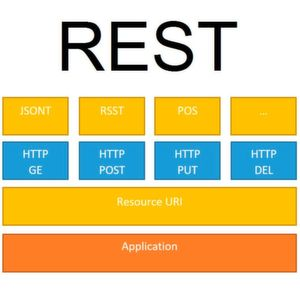
\includegraphics[scale=1]{images/REST_schichtenmodell.jpg}
    \caption{Rest Schichtenmodell (01.04.2020)}
    \url{https://images.vogel.de/vogelonline/bdb/1220900/1220968/4.jpg}
    \label{img:Rest_Schichtenmodell}
\end{figure}

\subsection{Elasticsearch [FK]}\label{sec:ES}

\begin{figure}[H]
    \centering
    
\includegraphics[scale=1]{images/ESLogo.PNG}
    \caption{Elasticsearch (01.04.2020)}
    \url{https://www.tudock.de/fileadmin/blog/blog_beitragsbilder/2018/Elasticsearch_-_Horizontal_Text_-_Full_Color_712.png}
\end{figure}
Elasticsearch ist eine in Java geschriebene Suchmaschine und zugleich NoSQL Datenbank. Es basiert auf der Volltextsuchmaschine Apache Lucene. Es ist eine dokumentenorientierte Datenbank und speichert die Dokumente im JSON [\ref{sec:json} Format. Diese Dokumente werden auch sofort indexiert um möglichst hohe Abfragegeschwindigkeiten zu ermöglichen. Der Suchserver kann als verteiltes System mit mehreren Rechnern betrieben werden und setzt damit auf eine hohe Verfügbarkeit und sehr gute Lastverteilung. „Elasticsearch zerteilt jeden Index [\ref{sec:Index}] in mehrere Stücke, so genannte shards (Scherben, Bruchstücke). Die shards eines Indexes können vom Anwender bei Bedarf auf mehrere Server (nodes) aufgeteilt werden (die Gruppe heißt Cluster), um die Rechenlast zu verteilen oder um Serverausfälle zu kompensieren. Läuft die Suchmaschine auf mehreren nodes, so wird einer als Master node der Gruppe bestimmt.“ \cite{PhysAufbau}
Neben Elasticsearch gibt es auch noch andere „gratis“ Volltextsuchmaschinen wie zum Beispiel der größte Konkurrent Apache Solr. Beide sind im Kern Open-Source Projekte haben aber ganz unterschiedliche Eigenschaften. Kurz die Unterschiede zusammengefasst ist Solr besser, wenn es um statische Daten geht aufgrund seiner Caches und Elasticsearch ist besser bei Logdateien und der Analyse von Daten. Ein detaillierter Vergleich würde hier den Rahmen sprengen, denn es geht ja um Elasticsearch. Wer dennoch einen genauen Vergleich will sollte sich diesen Artikel durchlesen: \cite{ESvsSolr}
\subsection{Abfragesprachen}
Die Standardabfragesprache von Elasticsearch ist „Query DSL“ (Domain Specific Language) welche auf JSON basiert um Abfragen durchzuführen. Elasticsearch bietet aber auch noch eine weitere Abfragesprache um es auch SQL gewöhnten Programmierern recht zu machen nämlich Elasticsearch SQL.
\subsection{Query DSL}
Grundsätzlich gibt es zwei verschiedene Abfragesprachen: „Leaf query clauses“ und „Compound query clauses“.
Bei Leaf queries wird nach einem bestimmten Wert in einem Feld gesucht.


Bei Compound query clauses werden Leaf und Compound abfragen so verpackt damit mehrere Abfragen auf logische Weise kombiniert werden können.
(vgl. \cite{ESQueryDsl}) 
\subsubsection{Relevance Score}
Die Relevanz Punktzahl gibt an wie wahrscheinlich jedes einzelne Dokument dem entspricht, was die Abfrage fordert. Die Zahl wird in jedem Dokument als meta Feld dargestellt ( \_score ). Jeder Abfragetyp bewertet den Score unterschiedlich. Außerdem hängt die Bewertung davon ab, ob die Abfrageklausel in einem Abfrage- oder Filterkontext ausgeführt wird. (vgl. \cite{DSLQueryFilter})
\subsubsection{Abfrage Kontext}
Im Abfrage Kontext wird überprüft wie gut ein Dokument auf die Aktuelle Abfrage zutrifft. Je nachdem wie gut das Dokument passt wird es als passend deklariert und die Relevanz Punktzahl ermittelt. Der Abfrage Kontext wird benutzt, wenn der „query“ Parameter in der Suche befüllt wird. (vgl. \cite{DSLQueryFilter})
\subsubsection{Filter Kontext}
Beim Filter Kontext wird überprüft, ob die Abfrage genau zutrifft. Bsp: Ist das „age“ Feld größer 60.
Es wird dabei keine Punktzahl bestimmt, sondern einfach mit Ja oder Nein bestimmt, ob das Dokument zu der Abfrage passt. Dies funktioniert natürlich am besten mit gut strukturierten Daten, um welche man sich selbst kümmern muss , da es ja eine schemafreie Datenbank ist. Ein weiterer Vorteil neben der klaren Ja/Nein Antwort ist das öfters ausgeführte Abfragen in einem Cache gespeichert werden, was wiederum die Performance stark erhöht.
Genutzt wird der Filter Kontext in Abfragen mit „filter“ oder „must/must\_not“ Parametern. (vgl. \cite{DSLQueryFilter})
\subsubsection{Beispielabfrage}
Folgendes Beispiel zeigt die Verwendung von Abfrage und Filter Kontexte. Dokumente welche folgenden Bedingungen erfüllen würden in der Suche gefunden werden.
\begin{itemize}
    \item Der Titel im Dokument enthält das Wort: „Search“.
    \item Das Inhaltsfeld enthält das Wort: „Elasticsearch“.
    \item Im „status“ feld steht nur „published“.
    \item Das Feld „publish\_date“ enthält ein Datum ab dem 1. Januar 2015.
\end{itemize}
\begin{figure}[H]
    \centering
    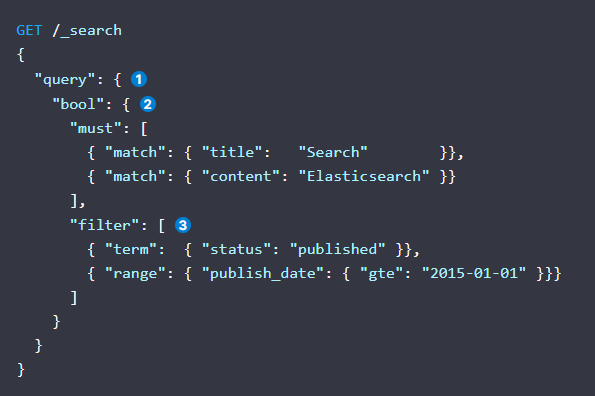
\includegraphics[scale=1]{images/ES_queryBsp.PNG}
    \caption{ES Beispielabfrage (01.04.2020)}
    \url{https://www.elastic.co/guide/en/elasticsearch/reference/current/query-filter-context.html}
    \label{img:ESexamplebsp}
\end{figure}
\begin{enumerate}
    \item Der „query“ Parameter zeigt den Kontext für die Abfrage an
    \item Die „bool“ und Die „match“ Klauseln geben an das es sich um einen query Kontext handelt. Somit wird die Relevanzpunktzahl für jeweilige Dokumente berechnet.
    \item Der „filter“ Parameter weist darauf hin, dass es sich um einen Filter Kontext handelt. Dokumente die nicht zu dem Filter passen werden aussortiert aber die Punktzahl vom query Kontext wird dabei nicht beeinflusst.
\end{enumerate}
Neben diesen Abfragen gibt es noch viele mehr aber das würde den Rahmen dieser kurzen Übersicht sprengen. (vgl. \cite{DSLQueryFilter})
\subsection{Elasticsearch SQL}
„Elasticsearch SQL ist eine X-Pack-Komponente, mit der SQL-ähnliche Abfragen in Echtzeit gegen Elasticsearch ausgeführt werden können. Ob über die REST-Schnittstelle, die Befehlszeile oder JDBC [\ref{sec:JDBC}], jeder Client kann SQL verwenden, um Daten innerhalb von Elasticsearch nativ zu suchen und zu aggregieren. Man kann sich Elasticsearch SQL als einen Übersetzer vorstellen, der sowohl SQL als auch Elasticsearch versteht und durch die Nutzung der Elasticsearch-Fähigkeiten das Lesen und Verarbeiten von Daten in Echtzeit und in großem Maßstab erleichtert." \cite{Elasticsearch-SQL}
\subsubsection{Vorteile}
Elasticsearch SQL ist nicht einfach eine Übersetzung in die DSL-Abfragesprache, sondern wurde entwickelt, um direkt auf die benötigten Nodes zugreifen zu können. Durch diese Integrierung ins System ist es auch nicht notwendig externe Hardware oder Libraries zu installieren. Außerdem schränkt Elasticsearch SQL die Suchfähigkeiten nicht ein. Aber der wahrscheinlich beste und offensichtlichste Vorteil ist die Möglichkeit, in einer gewohnten Sprache einfach Abfragen machen zu können ohne sich mit der DSL-Abfragesprache befassen zu müssen.
\subsubsection{Nachteile}
Neben mehreren kleineren Problemen bei größeren Mengen an Daten ist das größte Problem, das man seine gespeicherten Daten strukturiert halten muss oder zumindest sollte, wenn man das meiste aus der Sprache herausholen möchte. Somit wird der Verwaltungsaufwand erhöht.
\subsubsection{ES SQL Beispiel}
Anmerkung: Für dieses Beispiel verwende ich die Developer Konsole von Kibana \ref{ssec:devtools}.
Um Beispieldaten hinzuzufügen verwende ich bulk. Es werden drei Personen erstellt, welche die gleichen Eigenschaften besitzen.
\begin{figure}[H]
    \centering
    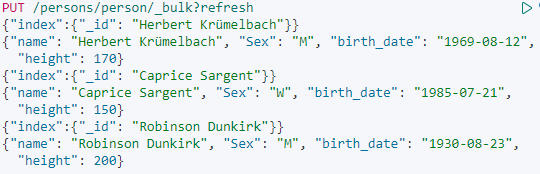
\includegraphics[scale=1.3]{images/es_sql_import.PNG}
    \caption{ES Beispiel Datenimport}
    \label{img:es_sql_import}
\end{figure}
Um nun eine Abfrage mit SQL zu machen, schreibt man einen POST Request mit dem Schlüsselwort „\_sql?format=txt“.
Außerdem benötigt man einen „query“ Parameter, in welchem die eigentliche SQL-Abfrage geschrieben ist. 
\begin{figure}[H]
    \centering
    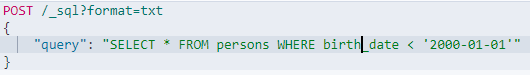
\includegraphics[scale=1.3]{images/es_sql_query.PNG}
    \caption{ES Beispiel Suche}
    \label{img:es_sql_query}
\end{figure}
Bei „format=txt“ wird dabei festgelegt, wie die Ausgabe aussehen soll. Im Falle von „txt“ wird das Ergebnis als Tabelle ausgegeben, wie wenn es direkt aus der Konsole kommen würde. Weitere Möglichkeiten sind: json, csv, yaml und noch mehr.
Nun zu der SQL-Abfrage: Nach dem „FROM“ Statement kommt der Index, in welchem gesucht werden soll. „birth\_date“ ist das Feld, das überprüft werden soll. Man merkt, das es ziemlich genau wie normales SQL agiert.
\begin{figure}[H]
    \centering
    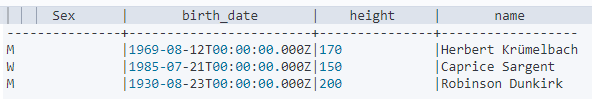
\includegraphics[scale=1.3]{images/es_sql_outputTxt.PNG}
    \caption{ES Beispiel Ergebnis}
    \label{img:es_sql_outputTxt}
\end{figure}
(vgl. \cite{EsSql})